
%%\documentclass{article}
\documentclass{scrartcl}

\usepackage{cmap}
\usepackage{booktabs}
\usepackage{colortbl}
\usepackage{multirow}
\usepackage{subfloat}
\usepackage{float}
\floatstyle{boxed} 
\restylefloat{figure}

\usepackage{lipsum}

\usepackage{kpfonts}

\usepackage{polyglossia}
\setdefaultlanguage{english}
%%%%%%%%%%%%%%%% for color
\usepackage{xcolor, colortbl} 
\newcommand{\mc}[2]{\multicolumn{#1}{c}{#2}}
\definecolor{Gray}{gray}{0.85}
\definecolor{LightCyan}{rgb}{0.88,1,1}

\newcolumntype{a}{>{\columncolor{Gray}}c}
\newcolumntype{b}{>{\columncolor{white}}c}
%%%%%%%%%%%%%%%%%%%%%%%%%%
%\usepackage[backend=biber]{biblatex}
\usepackage[backend=biber, style=ieee]{biblatex}
\addbibresource{plana.bib}

\usepackage{graphicx}
\graphicspath{ {images/} }






\begin{document}

\begin{titlepage}


\title{\textsc{\LARGE Bern University of Applied Sciences | BFH }\\[1cm]
\begin{center}
%
\includegraphics[width = 60mm]{logo.JPG}
\end{center}
\textsc{\small Department of Engineering and Information Technology}\\
\textsc{\small Project 2 (Module BTI7302) 20}\\[1cm]
\textsc{\small Report on  }\\
\textsc{"Planning of the Assignments Information System(PLANA)" Web Application}}
\date{\today}   %% or \date{01 november 2019}
\author{\textit{Author: }Kristina \textsc{Shiryagina} (\texttt{kristina.shiryagina@bfh.ch}) \\
 \textit{Supervisor: } Prof. Marcel \textsc{Pfahrer}  (\texttt{marcel.pfahrer@bfh.ch})\\
 }
\maketitle	

\newpage


	
\tableofcontents
\clearpage
\end{titlepage}

%%%%%%%%%% end title page
\setcounter{secnumdepth}{-2}% default for "report" is 2



\section{Acknowledgements}
I would like to thank my project supervisor - Prof. Marcel Pfahrer for his advice and guidance. 
I would also like to thank Andrei Herasimau for his corrections and Egger Samuel Sebastian for his advice.


\section{Abstract}
The focus of this project is to create the initial phase of a web application PLANA (Planning of assignments for lecturers) using ASP.NET Core Blazor.\\


To achieve this, the following has been done:
\begin{itemize}
\item Requirements Engineering
\item Domain Analysis
\item System Architecture and System Design
\item Research of  ASP.NET Core Blazor
\item Application Prototype
\end{itemize}

We measured the framework for popularity.\\

We came to the conclusion that ASP.NET Core Blazor is completely suitable for us.We have also created prototype for further work.


\setcounter{secnumdepth}{2}



\section{Introduction}

Nowadays we have a large selection of technologies for creating a web application. In the world of frameworks, advancements are made at a rapid rate. The most successful of frameworks are fast, facilitate the work of developers, add variety to a user interface, and improve technology as a whole. Our task as developers is to research these technologies, to try them out and use them.\\

Our goal is to create a web application for assignment planning for lecturers in our school. 
This work consists of two parts, - the project that is described in this document and the thesis which is planned as a continuation of this work in the next semester.
The project has several objectives:
\begin{itemize}
\item Employ software engineering techniques which include :
	\begin{itemize}
	\item Requirements engineering
	\item Domain Analysis
	\item System Architecture and System Design
	
	\end{itemize}
\item Research the ASP.NET Core Blazor framework, try it out and see if it suits us 
\item Create an application prototype

Why did we choose the ASP.NET Core Blazor framework for research and subsequent use?\\
ASP.NET Core Blazor is a framework for building interactive client-side web UI with .NET.  It has the following interesting features: \cite{blazor}
\begin{itemize}
\item alows creation of  rich interactive UIs using C\# instead of JavaScript
\item alows sharing of server-side and client-side application logic, which is written in .NET
\item alows rendering of UI as HTML and CSS for wide browser support, including mobile browsers.
\end{itemize}

The result of this work should be an accurate idea of which technologies will be used to create the web application, as well as which software engineering techniques should be utilized for the further implementation of the product.

\end{itemize}





\section{Customer Problem Statement}

\subsection{Problem Statement}
%\**
%A minimum 3-page high-level narrative about your project. The narrative should not be written from the developer’s perspective, describing the features of the planned system.
%Rather, put yourself into a customer’s role, and write your problem statement as if your imagined customer would write it! —Describe the problem that your customer is facing and his or her suggestions about how a software system could help.
%Your problem statement should be based on your project proposal, revised and improved as necessary.
%*\

Our plan is to create a system which will perform all the necessary functions for planning tasks for teachers in our school -  Berner Fachhochschule (BFH) . \\ 

The main users of this system are the study director and teachers. 
The study director will organize the planning of assignments for teachers and teachers will participate in this planning. Teachers will also manage their project information.

 It is a process, which involves the input of certain data for a specific user, certain views for each user, and time limits set by the system.



 Planning of assignments includes planning, managing and communication. These are all joint actions.
 
At our school, actual teacher assignment planning is done using Microsoft Excel tool.

 If we look at the requirements described above, we can clearly see that Excel is not the best option. We plan to substitute Excel with our own web application.
 Compares various Excel and web application we can clearly see that the web application is better suited to our requirements

\begin{table}[H]
\begin{center}
\begin{tabular}{| p{2.5cm}| p{6.5cm} |p{6.5cm}|}
\hline
\textbf{Features} & \textbf{Excel}& \textbf{Web Application} \\
\hline
\textbf{Enhanced accessibility(teamwork)}
   &              Sharing of excel spreadsheets can get out of control, there are many versions of the file. It is impossible to know who has made which changes. 
Excel is not designed for collaborative work.
& It is very important that with the web application, anyone who is authorized can access it. The administrator can specify who can use the application,
who can input data. Higher
granularity is possible, for example only exposing certain parts of a spreadsheet
do different user audiences.\\ \hline
\textbf{Support various devices}                   
&           Excel on IOS and Android isn’t so powerful as the PC version. For a
complex project, it is necessary to have a PC version.
	& Web applications easily support all the devices connected with
the internet. It’s also possible to use a smartphone to run web applications.\\ \hline
\textbf{Data storage}               
  &      Access to a spreadsheet is sometimes limited to one person at a time.
Spreadsheets have made a huge step forward due to the presence of Google Sheets.	
&  Databases have a more robust set of features for handling data. SQL
Server and Excel are in completely different weight classes in terms of data handling. SQL is a
more powerful tool. Databases are also better atprocessing enormous numbers of records.
 Databases work with different programming languages
, as opposed to Excel. Databases can be used by multiple users at the same
time.
Data is much safer in a database. \\ \hline
\textbf{Development (price, time)}
& Sometimes easy and cheaper to set up.
& Can have high development cost.
It takes some time to build the web application.\\ \hline
\end{tabular}
\end{center}
\caption{Comparing Excel to Web Application}
\label{table2}
\end{table}








A web application will allow us to implement features, like simultaneous system access by several users.
Users will receive only the specific views that they need, which will allow them to enter and confirm data without violating the integrity of the main data.

	
\subsection{Glossary}
\begin{itemize}


\item \textbf{FURPS+}\cite{eeles2005capturing} is a system for classifying requirements.
\begin{itemize}
\item Functionality
\item Usability
\item Reliability
\item Performance
\item Supportability 
\end{itemize}


\item \textbf{ SignalIR} is a free and open-source software library for Microsoft ASP.NET that allows server code to send asynchronous notifications to client-side web applications. 

\item \textbf{Blazor} is a free and open-source web framework that enables developers to create web apps using C\# and HTML. It is being developed by Microsoft.

\item \textbf{HTML} HyperText Markup language

\item \textbf{CSS} Cascading Style Sheets
\item \textbf{SQL} Structured Query Language
\item \textbf{JS } JavaScript
\item \textbf{CRUD} Create, read, update and delete
\item \textbf{EF} Entity framework
\item \textbf{UI} User Interface
\item \textbf{API} Application Programming Interface 

\item \textbf{MS} Microsoft
\item \textbf{BPMN} Business Process Model and Notation



\end{itemize}
\section{System Requirements}
 \subsection{Product Backlog and user stories}
    \begin{table}[H]
	\begin{center}
	\textbf{USER STORIES }\\[1cm]
	\begin{tabular}{| p{2.5cm}| p{4cm} | p{9cm} |}
	\hline
	\textbf{Id} & \textbf{Story Name} & \textbf{Story Description}\\
	\hline      
	\textbf{Study director} \\ \hline
	1.0 & Make a plan of assignments & As a study director, I want to be able to make a concrete plan of assignments for lecturers for the coming year as well as a provision plan for the next 2-3 years, so the teachers can be better informed about their work hours and schedule for the next several years. And it will be easier to add new small changes into the employment plan. \\ \hline
	2.0 & Manage plan of assignments & As a study director, I want to be able to manage information in the assignment's plan, so that I am able to change the information.\\ \hline
	\textbf{Future user stories} \\ \hline
	3.0 & Get projects information & As a study director, I want to see which lecturers supervise which students in students  projects like project1, project2, bachelor thesis, master thesis, so I can use this information for managing processes. \\ \hline
	\textbf{Lecturer} \\ \hline
	4.0 & See the plan of my assignments &  As a lecturer, I want to see my assignment's plan for this year and next two years, so that I know the timetable of classes and I can manage my time better.
\\ \hline
	5.0 & Participate in the planning and management of assignments &   As a lecturer, I want to participate in the planning of assignments, so I can add my proposal for the plan and confirm it.\\ \hline
	6.0 & Manage projects & As a lecturer, I want to be able to manage my projects, so I can easily change any kind of information on my project. (e.g.  add student/s to my projects, I know which student(s) is/are working on which project(s)).\\ \hline
	
     \end{tabular}
	\end{center}
	\caption{Product Backlog}
	\label{table2}
	\end{table}
	
	
 The system has been provided with a list of requirements. All requirements are based on consumer needs. There is an identifier in the form of REQ-x and a priority weight from 1 to 5. A higher priority weight indicates that the corresponding requirement is more important for the project's success and for meeting customer needs.
\subsection{Enumerated Functional Requirements}
\begin{table}[H]
\begin{center}
\begin{tabular}{|p{2.5cm} |p{7.5cm} | p{2.5cm} | }
\hline
\textbf{}  & \textbf{Description} & \textbf{Priority Weight}\\
\hline
REQ1 & The system shall allow the study director to make a plan of assignments, e.g. a concrete plan for the coming year as well as a provisional plan for the next 2-3 years      		&  5 \\ \hline
REQ2  &    The system shall allow the lecturer to participate in the creation of the plan, i.e. manage his own assignments..        	& 5 \\ \hline
REQ3  &    The system shall allow the study director to manage assignment plan.       	&5\\ \hline
REQ4   &      The system shall allow the lecturer to manage his projects like project1, project2, bachelor thesis, master thesis     		& 4 \\ \hline
REQ5   &      The system shall allow the lecturer to see his assignment plan for the coming year and provisional for next 2-3 years     		& 5\\ \hline

REQ6   &       While the user types a question, the system will be able to compare the search string to existing questions and prompt the user to look at those 		& 1\\ \hline
REQ7                &   The system should show the study director the maximum number of working hours for a given lecturer    	&  1\\ \hline
REQ8                &     The System should allow the  study director to copy assignment plan from one year to other years, from one semester to another        	&  2\\ \hline
REQ9            &   The system should offer possible replacements of the lecturer in case of sabbaticals and in other special cases       	& 1\\ \hline


\end{tabular}
\end{center}

\caption{Functional Requirements}
\label{table2}
\end{table}
\subsection{Enumerated Non-Functional Requirements}
Non-functional requirements are based on FURPS+, which stands for \textbf{functional usability, reliability, performance, supportability}, and other attributes.
These requirements  mainly pertain to quality attributes such as capability, compatibility, security, responsiveness, availability, efficiency, and maintainability.


\begin{table}[H]
\begin{center}
\begin{tabular}{| p{2.5cm}| p{7.5cm} |p{2.5cm}|}
\hline
\textbf{FURPS+}
\textbf{} & \textbf{Description}& \textbf{Priority Weight} \\
\hline
REQ11                    &       The system shall have an almost constant uptime.      	&  5 \\ \hline
REQ12                   &      The search engine shall be reliable and will return relevant and accurate results.       	&  2 \\ \hline
REQ13                   &         The system should be easy to navigate and utilize.    	&  2 \\ \hline
REQ14                    &         The system must be  supported by different browsers, on both web and mobile platforms  	& 1\\ \hline
%REQ                    &              	&  \\ \hline
%REQ                   &             	& \\ \hline
%REQ                    &              	&  \\ \hline
%REQ                    &              	&  \\ \hline
%REQ                   &             	& \\ \hline
%REQ                    &              	&  \\ \hline
%REQ                    &              	&  \\ \hline
%REQ                   &             	& \\ \hline
\end{tabular}
\end{center}
\caption{Non-Functional Requirements }
\label{table2}
\end{table}



%\subsection{User Interface Requirements}

   

        
     


\section{Functional Requirements Specifications}
 	\subsection{Stakeholder Summary}
 	The stakeholders of our system are:
  	\begin{itemize}
  	\item \textbf{ Study director}\\
  	The first major stakeholder is a study director.The study director can be both the person who makes an assignment plan and also a lecturer. 
  	
  	\item  \textbf{ Lecturer} \\
  	The lecturer is another major stakeholder of our system. He participates in assignment planning, manages his projects and he uses the system to be informed of his assignment plan.
  	
  	\item  \textbf{ Institute Manager} \\
  	The institute manager is a stakeholder of our system. He organises the planning of research projects.
  	\end{itemize}
  	
  	\subsection{Actors and Goals}
  	The roles of people that will directly interact with the system and their goals.
  	
%%%%%%%%%%%%%  actor study director 	
  \begin{itemize}
  \item \underline{\textbf {actor} -Study director}
	
  		\begin{itemize}
  			\item Initiating Actor
  			\item \textbf{goal} Uses  system to make a plan of assignments for lecturers. 
  			
  		\end{itemize}
  	
%%%%%%%%%%%%   actor lecturer	
 \item \underline{\textbf {actor} -Lecturer} 
		\begin{itemize}
		\item Initiating Actor
		\item  \textbf{goal }Uses the system to participate in the planning of  his assignments .
		    \item  \textbf{goal }Uses the system to get his assignment plan .
		    \item \textbf{goal} Uses the system to manage his assignments.
  			\item \textbf{goal }Uses the system to  manage his projects.
  	
\end{itemize}    	


 
\end{itemize}   

 \subsection{Business Process Model and Notation(BPMN)}
 In this section, we show a graphical notation of the Planning of assignments process. The model in Figure 1 is provided to make this process easier to understand. 
 
 \begin{figure}[h]
\centering
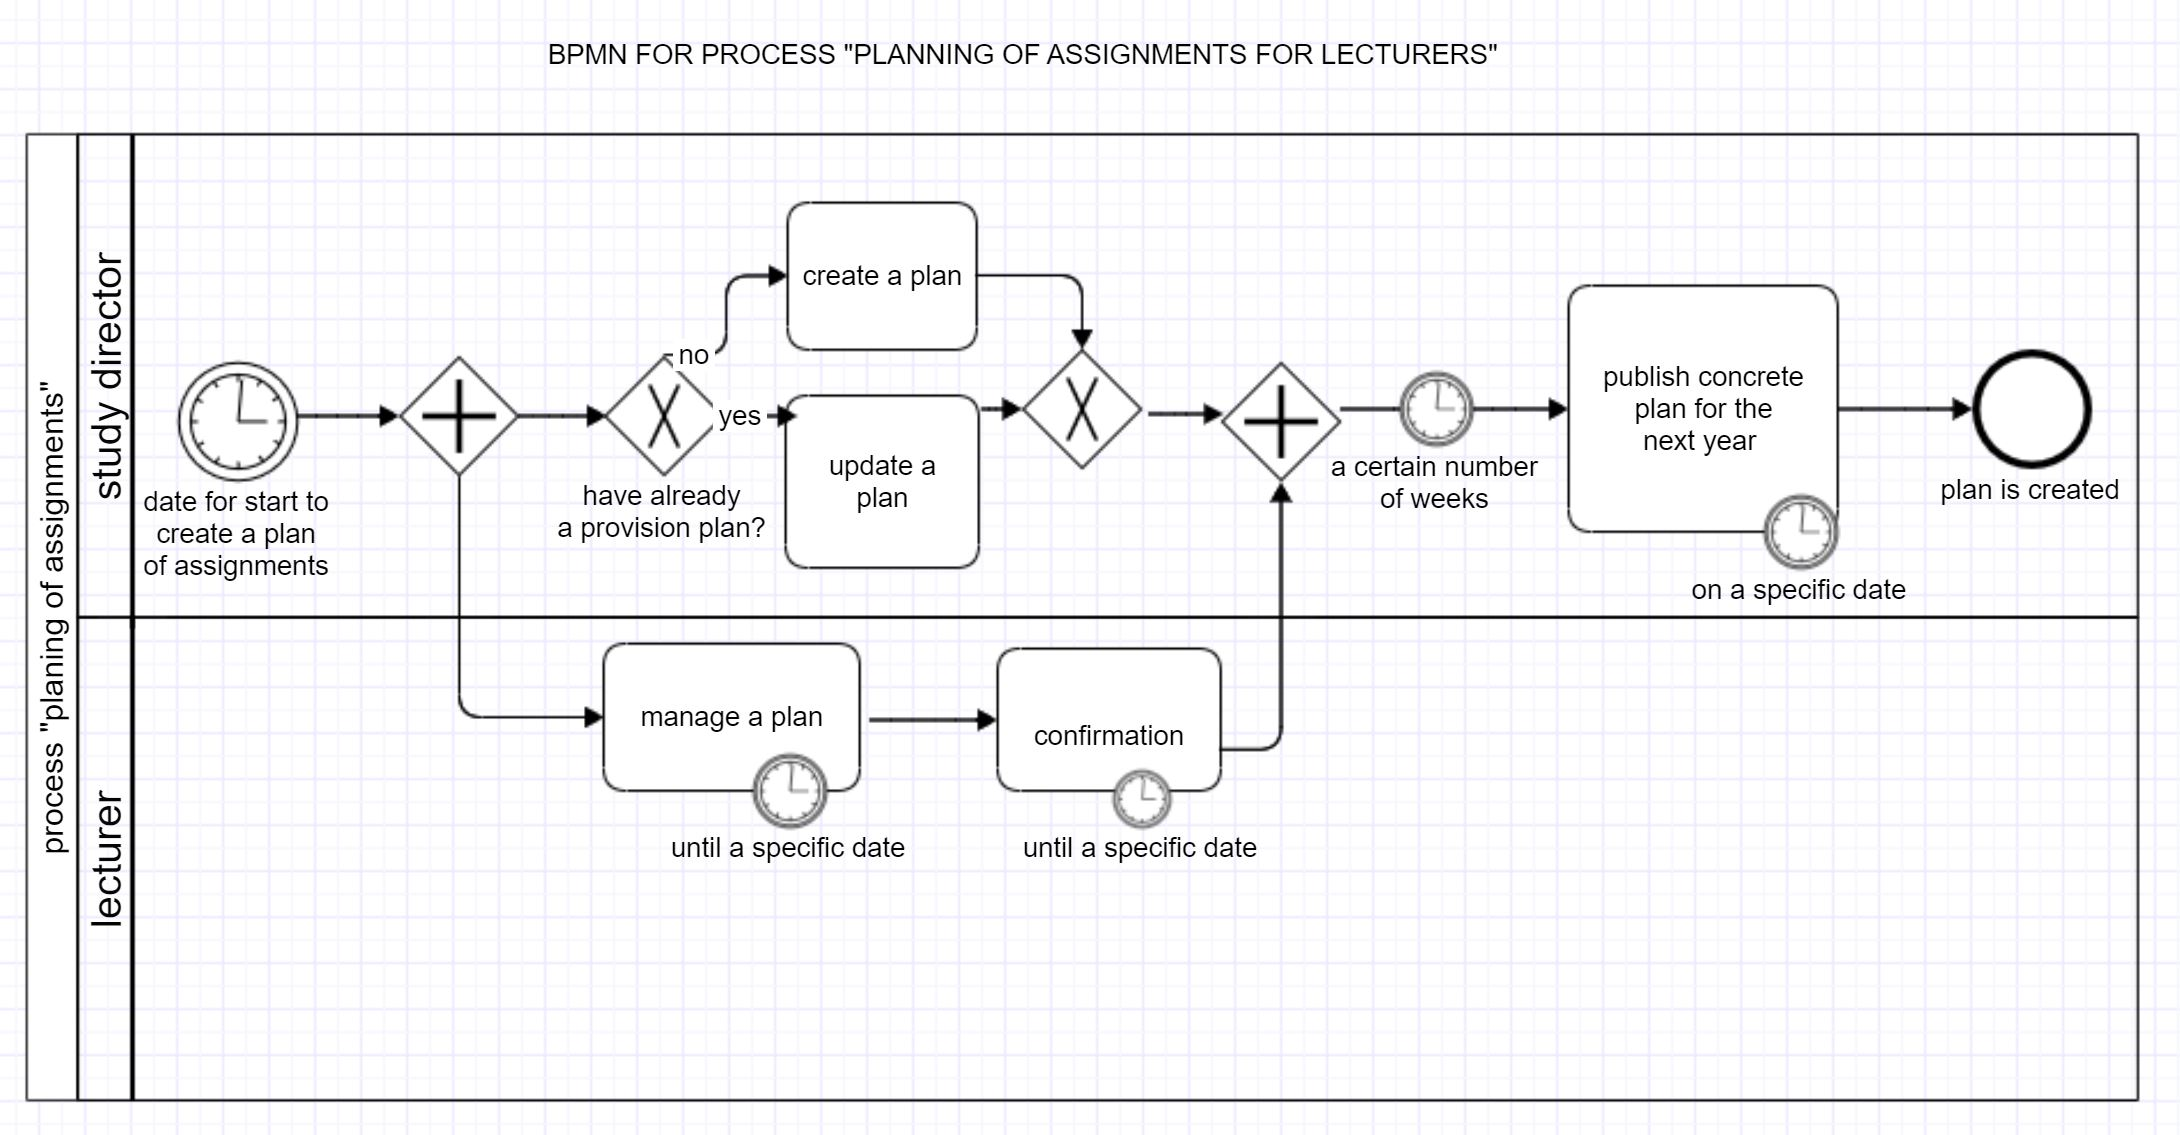
\includegraphics[width=150mm]{uml/bpmn.JPG}
\caption{BPMN of "Creating a plan of assignments" 1st version}
\label{blabla}
\end{figure}

In Figure 1, we show the process of creating an assignment plan and also the interaction between the study director and lecturer. \\
The main process of creating an assignment plan shall start at a certain date. As we can see from this diagram, it is a collaborative job.The study director creates a plan with all the necessary details or updates a plan that already exists. At the same time, the lecturers shall manage their assignment plan. \\
The lecturers shall manage their plan until a specific date. Then, the study director makes some last changes, after which each teacher checks his plan and confirms it until a certain date.\\
After a certain period of time, the exact assignment plan is published.
\\
After analyzing this model, we came to the conclusion that small changes in it will result in greater clarity in the process. Another minor change is the addition of messages to start certain processes.
 
 \begin{figure}[h]
\centering
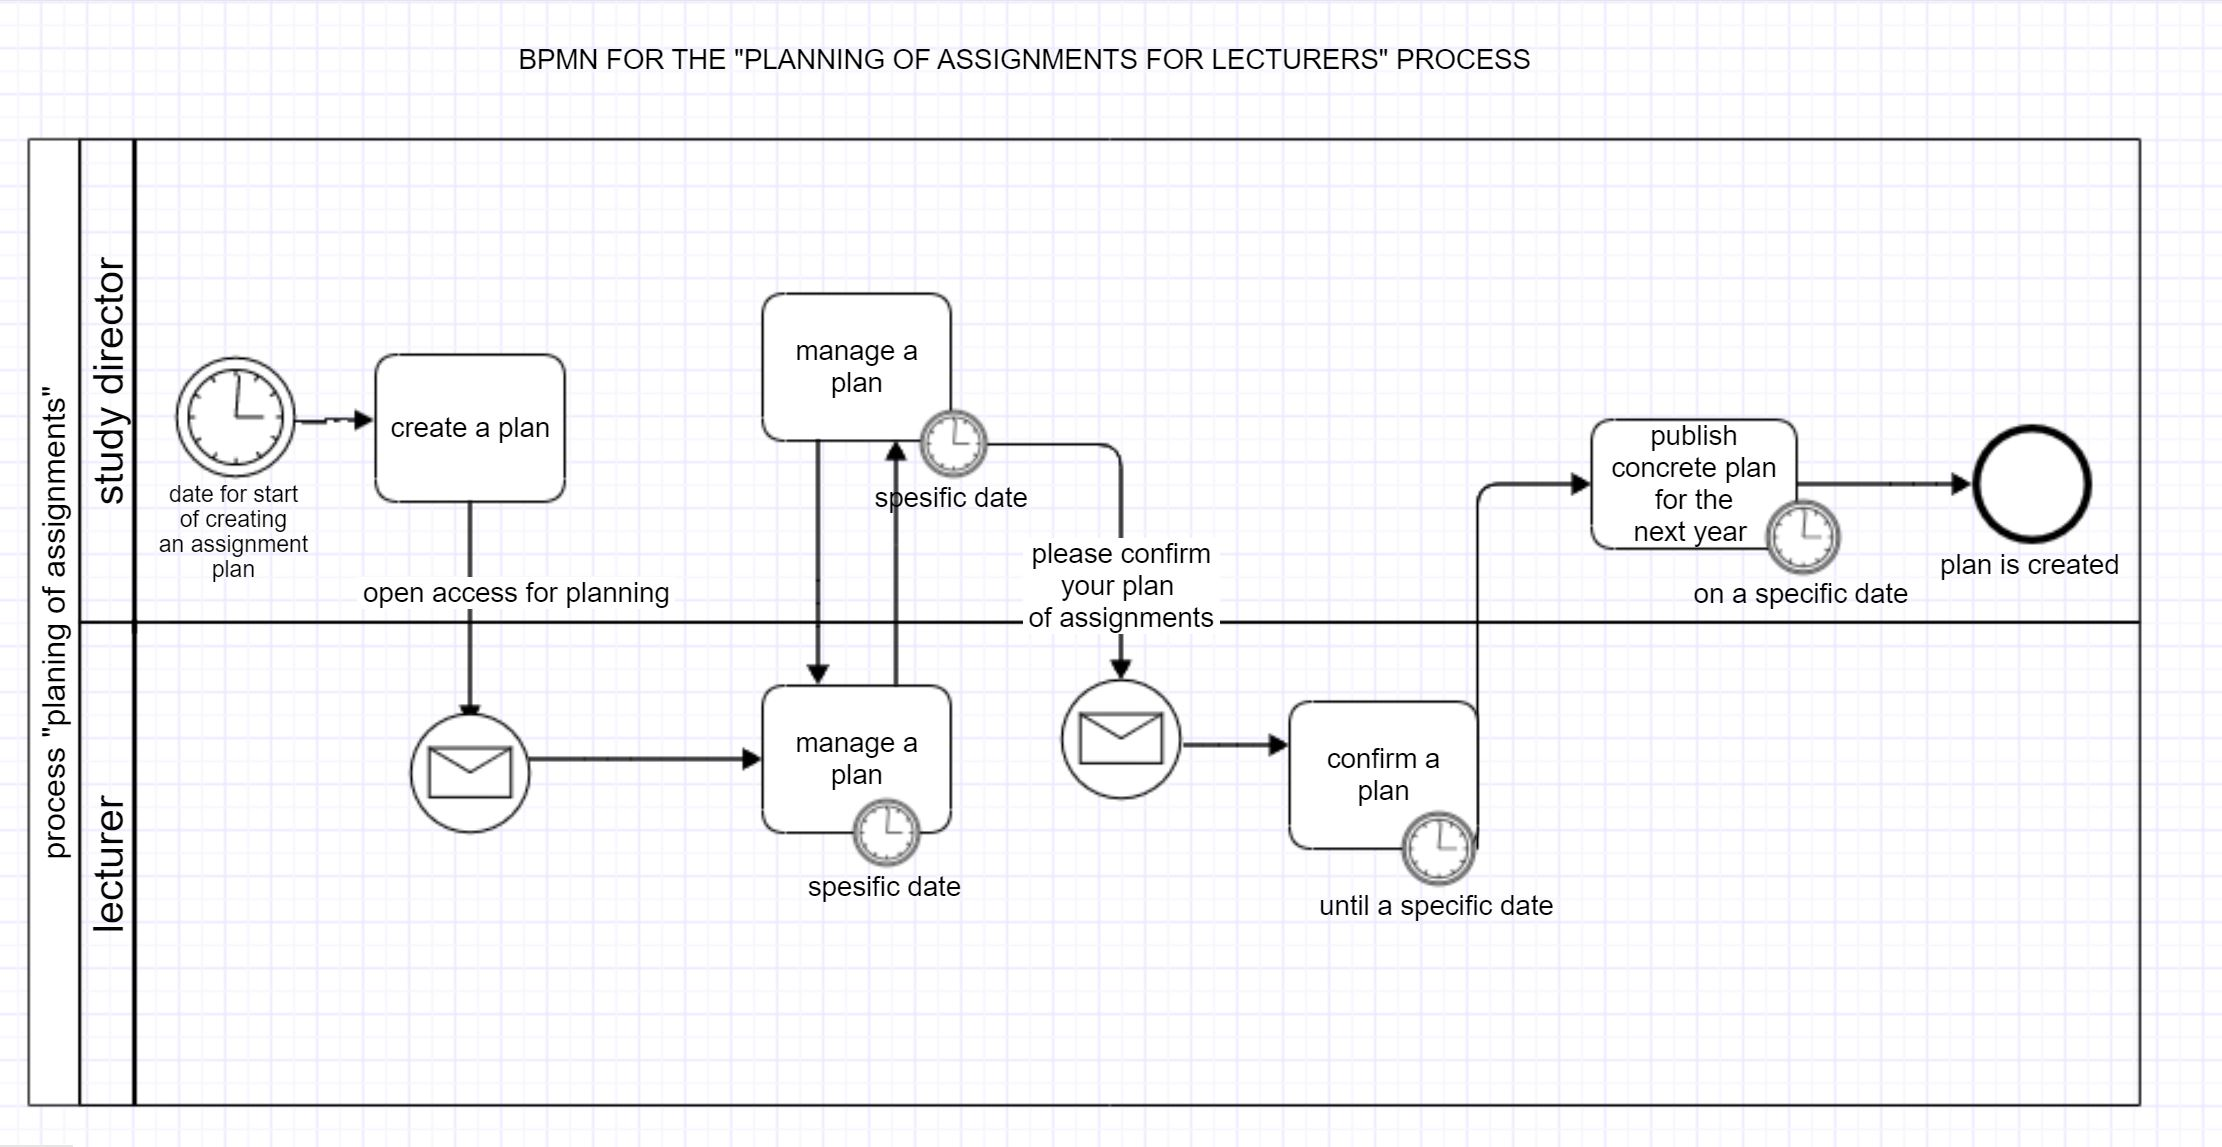
\includegraphics[width=150mm]{uml/bpmn2.JPG}
\caption{BPMN of "Creating a plan of assignments" 2nd version}
\label{blabla}
\end{figure}

Unlike the first version, in Figure 2 it is clear that the director starts the planning process, then joint work on planning takes place, which is completed by a certain time, and then the plan is confirmed and published by a certain date. 


  	\subsection{Use Cases}
  	\subsubsection{ i \& ii. Casual and Fully-Dressed Descriptions}
  	
\textbf{\underline{UC\#1.1 Create a concrete plan} }   \\
 The Study director can create a concrete assignment plan of lecturers for the coming year.    \\
  
 
\begin{table}[H]
\begin{center}
\begin{tabular}{| p{2.5cm}| p{12.5cm} |}
\hline
\textbf{UC\#1.1 } & \textbf{Use case description of "Create a concrete plan" } \\
\hline
Name  & Create  a concrete plan .\\ \hline
	         Summary  & The Study director makes a concrete assignment plan for  lecturers for the coming year . \\ \hline
	         Actor   & The Study director and The Lecturer\\ \hline
	         Precondition & The Study director and The Lecturer have logged into the PLANA information system. \\ \hline
	         Description & 
	         
	         \begin{enumerate}
	   		\item The Study director opens a assignment plan
			\item If there is no provisional plan, create a new plan 
				\begin{itemize}
				\item for each lecturer:
				\item  adds module runs . 
				\item adds a percentage/part of employment for concrete module run.
				\item add additional assignments :
				           \begin{itemize}
			 			 \item Teaching obligations in other departments and schools (e.g. further education, MSE, ...)
			 			 \item Administrative and managerial activities
			  			\item Research projects
			 			
			 			   \item In case of sabbaticals(research semester), adds it 
			 		 \end{itemize}
			
				
				\end{itemize}
				\item if a provisional plan exists, then just update it
			\item at the same time, wait for input from lecturer's side (lecturers participated in creating plan),  they manage their assignments.
			\item after the lecturers have confirmed the plan,the study director publishes the plan on a certain date
			                
			\end{enumerate}
	             \\ \hline	        
%	          Alternatives  & . \\ \hline
	          Postcondition &   Concrete plan of assignments for lecturers is created for coming year. \\ \hline
	           
\end{tabular}
\end{center}
\caption{ UC\#1.1 Create a concrete plan}
\label{table2}
\end{table}
			
			
			 	 
			
			  

			

%%%%%% uc1.2
\textbf{\underline{UC\#1.2 Create a provisional plan }  }    \\ 
  Study director  can create a provisional assignment plan for lecturers for the next 2-3 years.      	\\
  
  \begin{table}[H]
\begin{center}
\begin{tabular}{| p{2.5cm}| p{12.5cm} |}
\hline
\textbf{UC\#2 } & \textbf{Use case description of Create a provisional plan} \\
\hline
Name  &  Create a provisional plan .\\ \hline
	         Summary  &The Study director makes a provisional assignment plan for  lecturers for the the next 2-3 years . \\ \hline
	         Actor   &The Study director  and the Lecturer \\ \hline
	         Precondition & Study director and the Lecturer have logged into the PLANA information system. \\ \hline
	         Description & 
	         \begin{enumerate}
	   		\item The Study director opens assignment plan.
			\item Makes a copy of concrete plan from one Semester to another one  :
			       \begin{itemize}
			       \item chooses assignment plan of modules or whole assignment plan and copies it to another Semester .
			   
			       \end{itemize}
			\item Or manually makes  plan for the next year.    
			\item  In the same time Lecturer opens his own plan of assignments 
			\item  Check the assignment plan 
			\item Manages his assignments and confirms it.
			
			\item The same procedure for other semesters, so that study director has a plan for the next 2-3 years.
			\end{enumerate}
	             \\ \hline	        
%	          Alternatives  & . \\ \hline
	          Postcondition &   Provisional assignment plan for lecturers is created for the next 2-3 years.  \\ \hline
\end{tabular}
\end{center}
\caption{ UC\#1.2 Create a provision plan}
\label{table2}
\end{table}	          
	          
	\newpage          
	          
%%%%%%%% uc1.3

\textbf{\underline{UC\#1.3  Manage plan}}  \\
The Study director and the Lecturer can manage an assignment plan. This includes adding, changing or deleting information in the assignment plan.   \\ 

\begin{table}[H]
\begin{center}
\begin{tabular}{| p{2.5cm}| p{12.5cm} |}
\hline
\textbf{UC\#1.3 } & \textbf{Manage plan } \\
\hline
Name  &  Manage plan .\\ \hline
	         Summary  & The Study director and the Lecturer can manage plan of assignments for lecturers. \\ \hline
	         Actor   & The Study director and the Lecturer \\ \hline
	         Precondition & The Study director and the Lecturer  have logged into the PLANA information system. \\ \hline
	         Description & 
	         \begin{enumerate}
	   		\item Open assignment plan
			\item Adds /deletes/updates information in it.
			
			\end{enumerate}
	             \\ \hline	        
%	          Alternatives  & . \\ \hline
	          Postcondition &  Plan has been changed.\\ \hline
	           
\end{tabular}
\end{center}
\caption{UC\#1.3  Manage plan}
\label{table2}
\end{table}

%%%%%%%%  uc1.3.1
\textbf{\underline{UC\#1.3.1 View plan}}\\
The Lecturer can see his own plan for the next 2-3 years.

\begin{table}[H]
\begin{center}
\begin{tabular}{| p{2.5cm}| p{12.5cm} |}
\hline
\textbf{UC\#5 } & \textbf{Use case description of "View plan" } \\
\hline
Name  & View plan.\\ \hline
	         Summary  & The Lecturer sees his own assignment plan. \\ \hline
	         Actor   & The Lecturer. \\ \hline
	         Precondition &  The Lecturer has logged into the PLANA information system. \\ \hline
	         Description & 
	         \begin{enumerate}
	   		\item Opens assignment plan.
			\item Sees all modules, additional assignments and other information about assignments for the next 2-3 years.
			
		
			
			\end{enumerate}
	             \\ \hline	        
%	          Alternatives  & \\ \hline
	          Postcondition &  Lecturer has seen the assignment plan for the next 2-3 years. \\ \hline
	          
\end{tabular}
\end{center}
\caption{UC\#1.3.1 View plan}
\label{table2}
\end{table}

\pagebreak
%%%%%%% uc2

 \textbf{\underline{UC\#2  Manage  project information}}    \\ 
 A lecturer can manage project information. This includes adding or deleting project information like information about which students work on which project. \\

\begin{table}[H]
\begin{center}
\begin{tabular}{| p{2.5cm}| p{12.5cm} |}
\hline
\textbf{UC\#2 } & \textbf{Use case description of "Manage projects information" } \\
\hline
Name  & Manage projects information.\\ \hline
	         Summary  & The Lecturer adds students to his projects \\ \hline
	         Actor   & The Lecturer. \\ \hline
	         Precondition & The Lecturer has logged into the PLANA information system. \\ \hline
	         Description & 
	         \begin{enumerate}
	   		\item Open project list.
			\item Add/delete/update information about projects.
			
			\end{enumerate}
	             \\ \hline	        
%	          Alternatives  & . \\ \hline
	          Postcondition &   Project information has been changed. \\ \hline
	           
\end{tabular}
\end{center}
\caption{UC\#2  Manage  project information}
\label{table2}
\end{table}
  	

%%%%%%%% uc6
%
% \textbf{\underline{UC\#6  Planning of  additional assignments}}    \\ 
% Study director ,  Lecturer  and Institute manager  can manage additional assignments.  \\
%
%\begin{table}[H]
%\begin{center}
%\begin{tabular}{| p{2.5cm}| p{12.5cm} |}
%\hline
%\textbf{UC\#6 } & \textbf{Use case description of Planing  of additional assignments} \\
%\hline
%Name  & Manage additional assignments.\\ \hline
%	         Summary  &  \\ \hline
%	         Actor   & Study director, Lecturer, Institute Manager\\ \hline
%	         Precondition & Study director, Lecturer  and Institute Manager have logged into the PLANA information system. \\ \hline
%	         Description & 
%	         \begin{enumerate}
%	   		\item 
%			\item 
%			\item 
%			\end{enumerate}
%	             \\ \hline	        
%	          Alternatives  & . \\ \hline
%	          Postcondition &   Additional assignments have been panned. \\ \hline
%	           
%\end{tabular}
%\end{center}
%\caption{.}
%\label{table2}
%\end{table}
%  	
  	
 
 \pagebreak
  	
  	\subsubsection{ iii Use Case Diagram}
  	
  	Figure 3 shows the use cases of our system.
  	  	\begin{figure}[H]
\centering
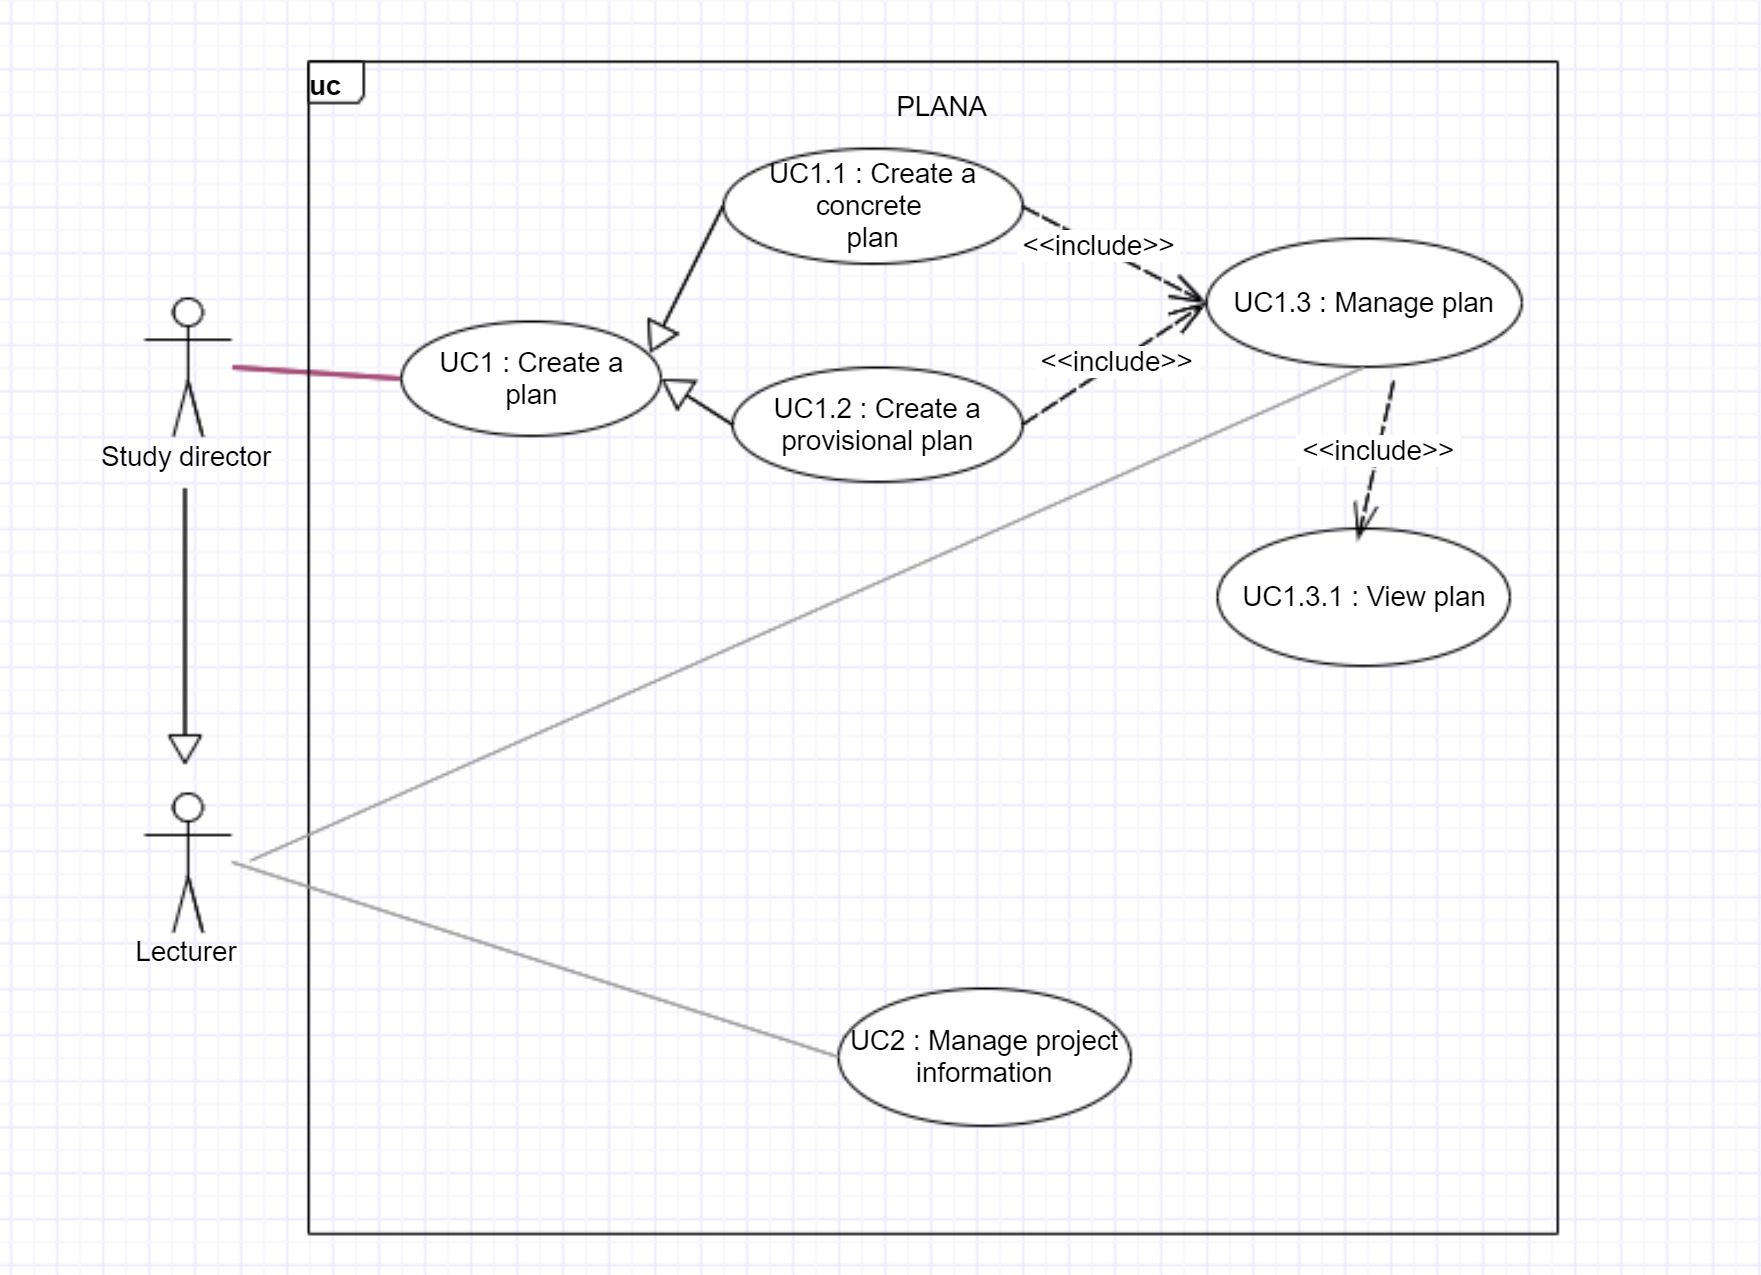
\includegraphics[width=150mm]{uml/ucd_last_last.JPG}
\caption{Use Case Diagram for the Study director and the Lecturer }
\label{ucd_study director&lecturer}
\end{figure}
    
    
  \pagebreak
  	
\section{Domain Analysis} 	 
    \subsection{Domain model}  
 The domain model (Figure 4) shows us the important concept classes, associations and multiplicities between them.
    \begin{figure}[H]
\centering
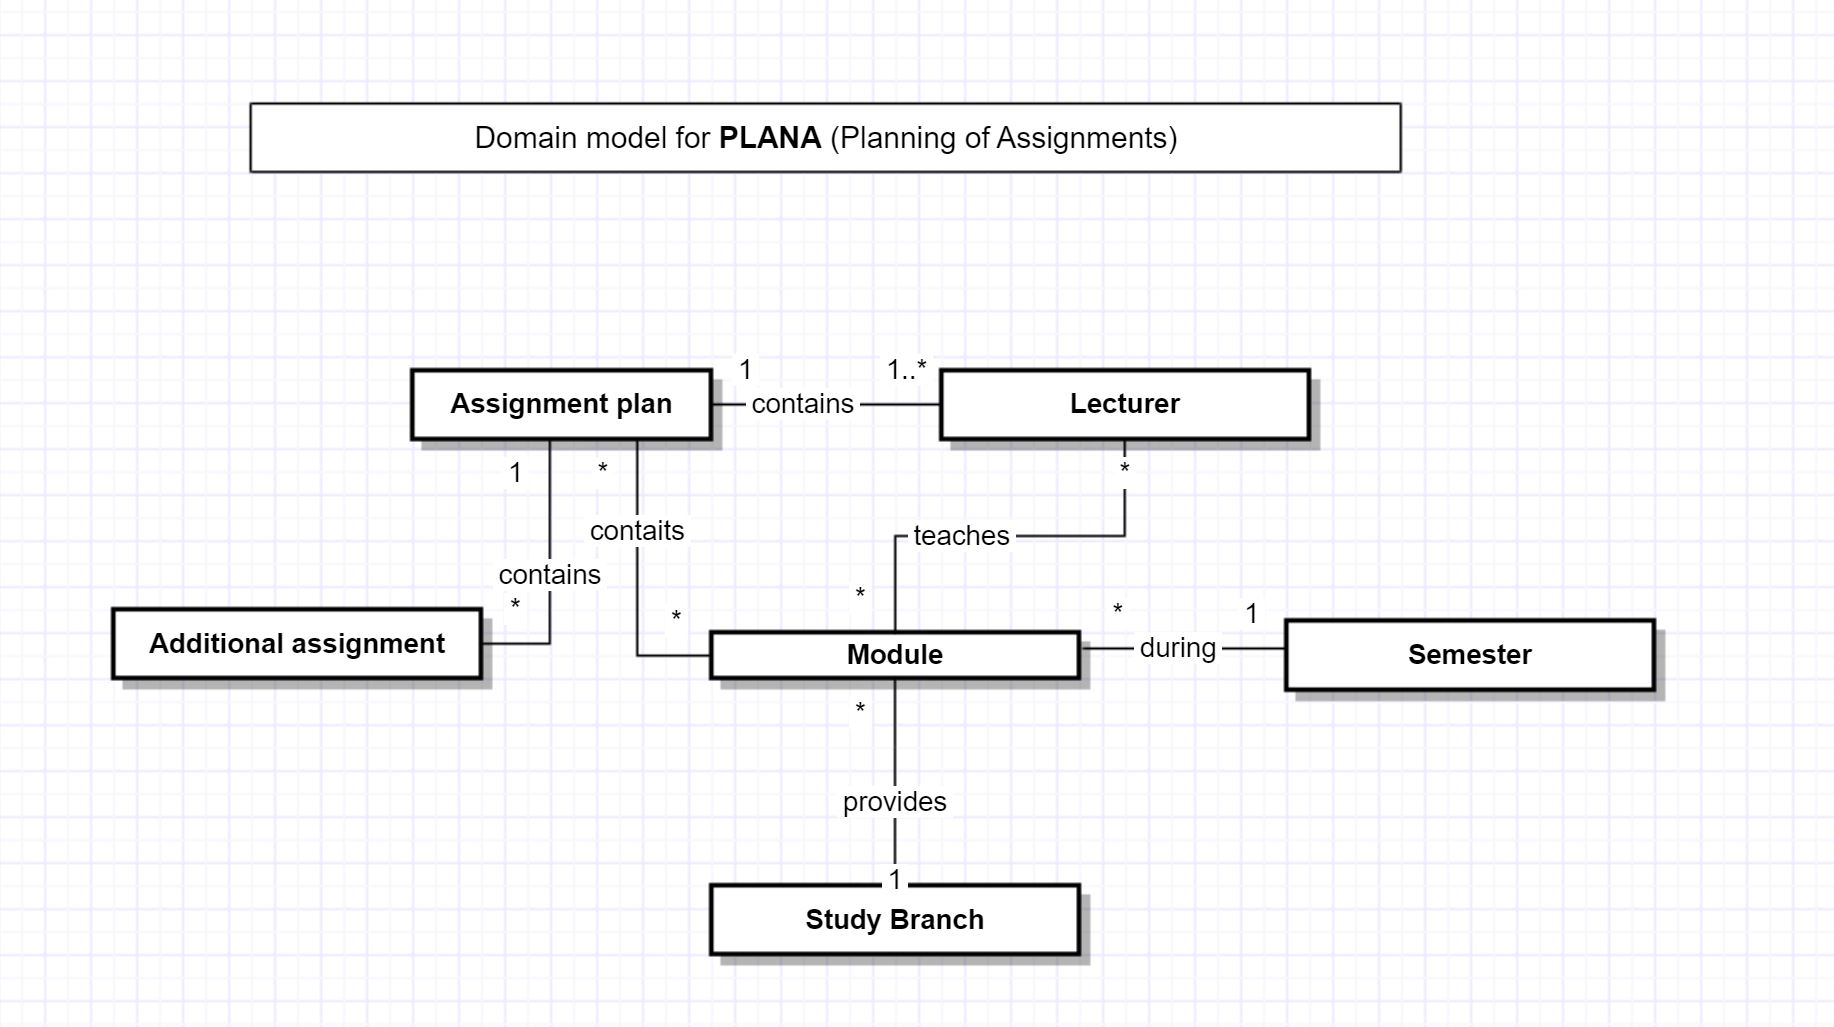
\includegraphics[width=150mm]{uml/domain3}
\caption{Domain model for  PLANA}
\label{Domain model  1st verstion}
\end{figure} 

Figure 5 depicts an updated version of the domain model. In the second version of the domain model, we have made several changes. We deleted the concept class "assignment plan" and we have connected lecturer with the module run and the additional assignments. 
\begin{figure}[H]
\centering
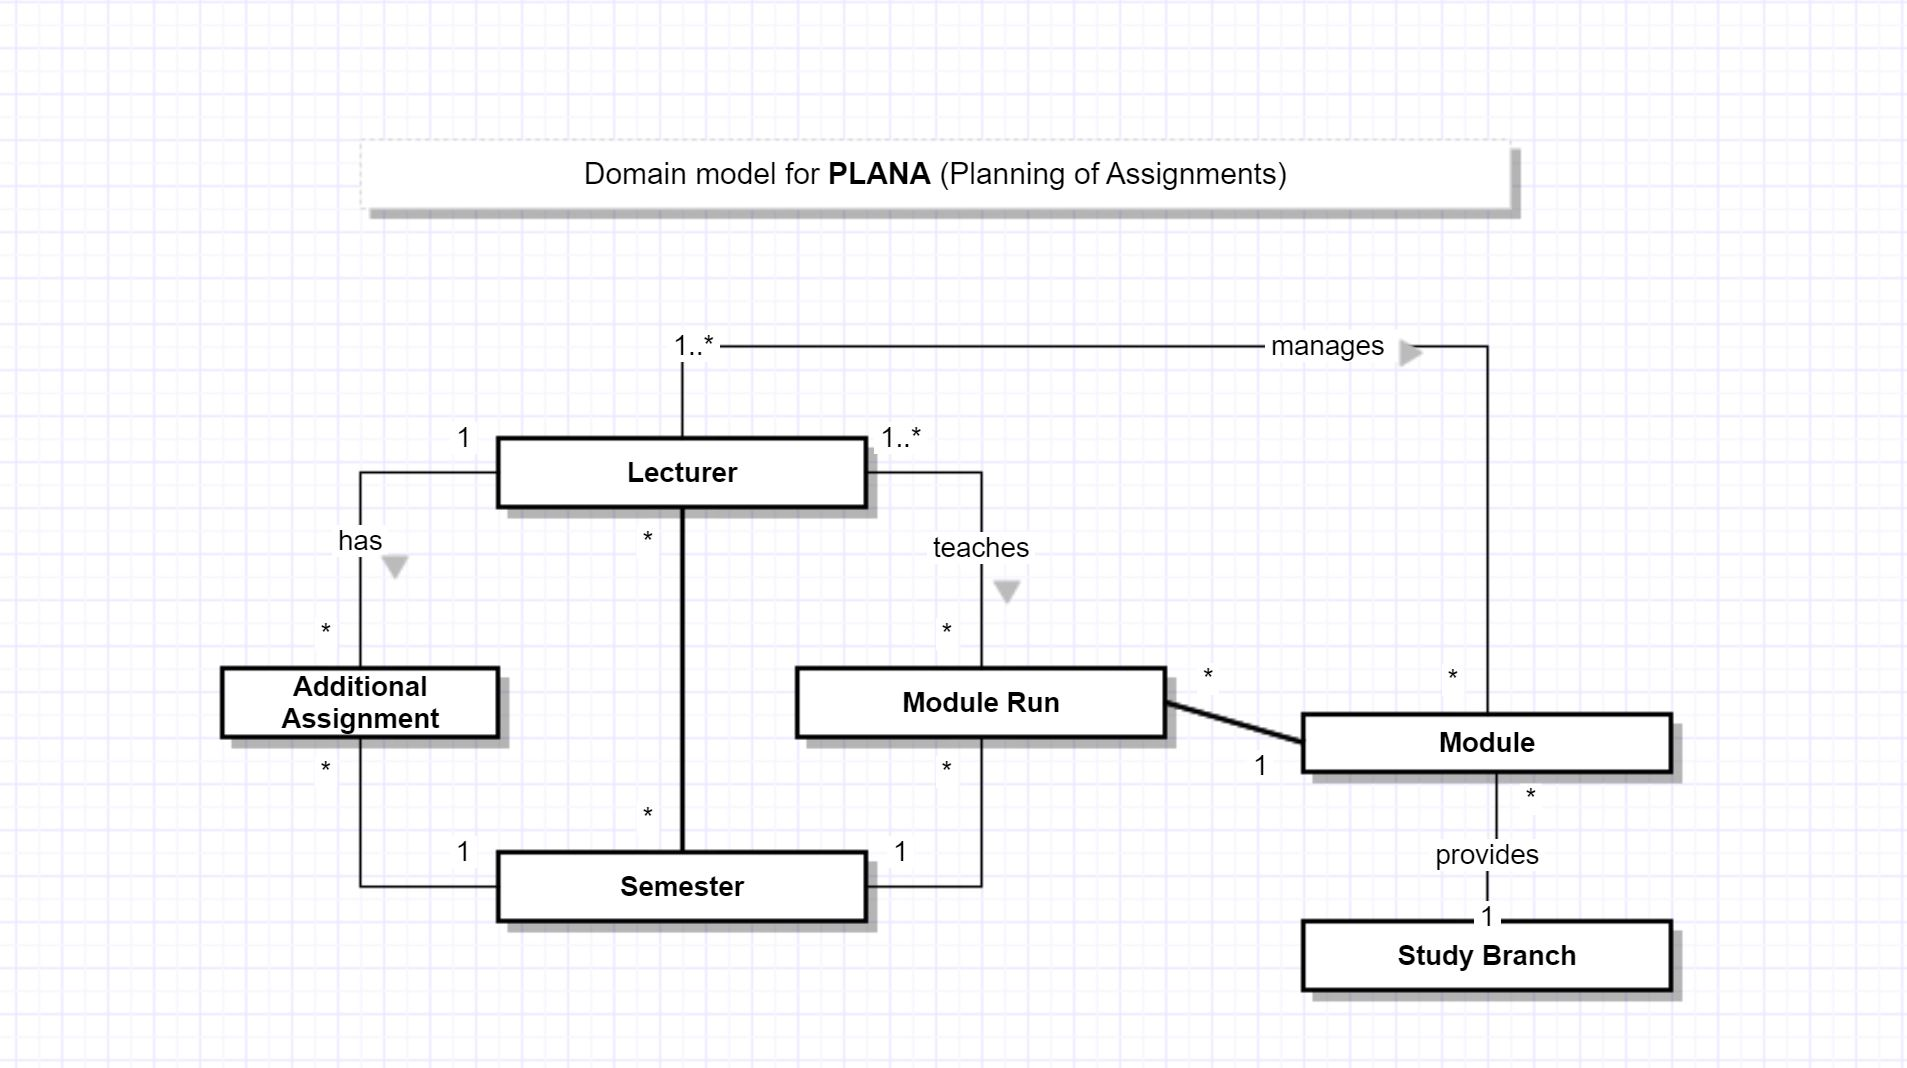
\includegraphics[width=150mm]{uml/domain_last}
\caption{Domain model for  PLANA}
\label{Domain model 2nd version}
\end{figure} 

Figure 6 depicts a domain model with attributes

\begin{figure}[H]
\centering
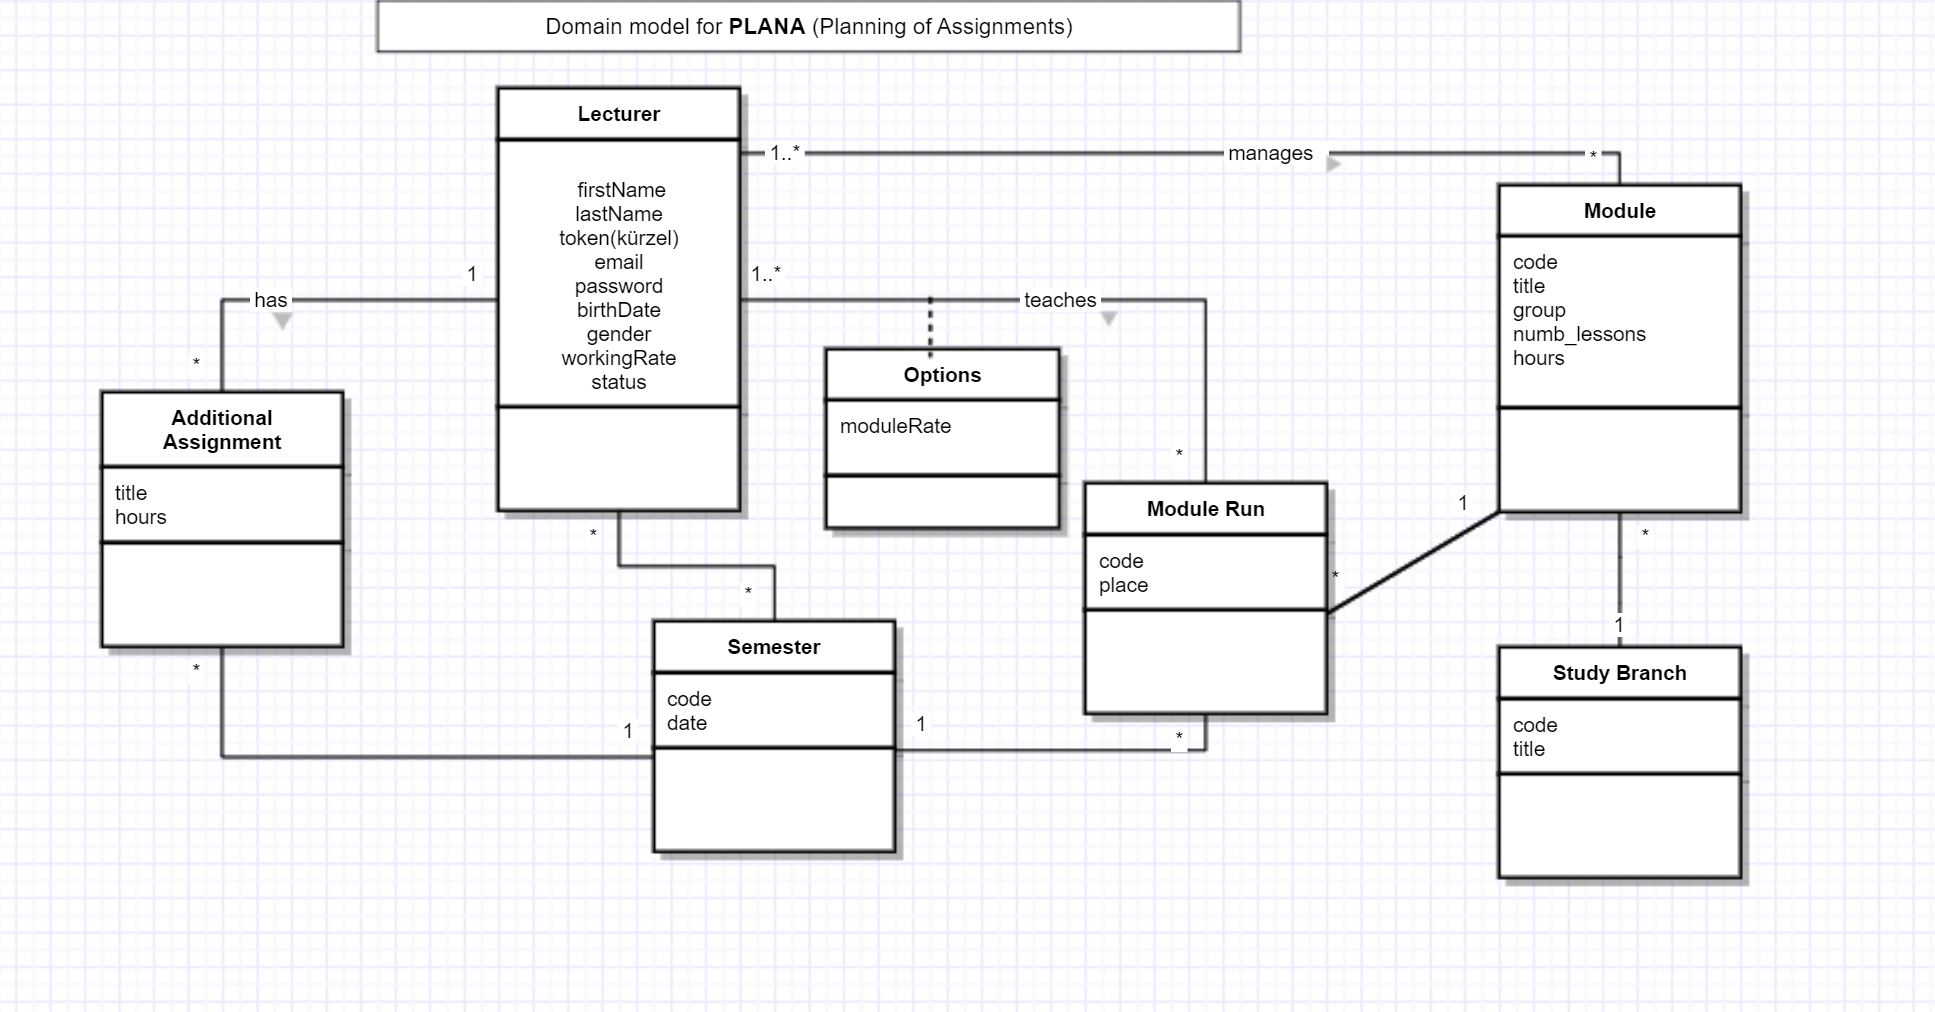
\includegraphics[width=150mm]{uml/domain_attributes}
\caption{Domain model for  PLANA}
\label{Domain model  with attributes}
\end{figure} 


	    \subsubsection{i. Concept Definition}
	    
	    \begin{itemize}
	    \item Concept class \textbf{Lecturer} models a person who teaches in a school.
	     \item Concept class \textbf{Study Branch} models a conceptual subdivision of subjects that form a study programme.
	      \item Concept class \textbf{Module} models a set of independent units that form a course at the school.
	       \item Concept class \textbf{Module Run } models executions of a course in different languages.
	       	      \item Concept class \textbf{Additional Assignment} models a set of independent units that form an additional task for the assignment's plan for the lecturer.
  \item Concept class \textbf{Semester} models the periods in the year, during which the lecturer is present in the school.
	         
	    \end{itemize}


	      
	    
	    \subsubsection{ii. Association Definition}
	    \begin{table}[H]
\begin{center}
\begin{tabular}{| p{6.5cm}| p{6.5cm} |p{2.5cm}|}

\hline
\rowcolor{LightCyan}
\textbf{Concept Pair} & \textbf{Association Definition}& \textbf{Association Name} \\
\hline
Lecturer -> Module Run                    &    Lecturer can teach zero or        more Module Runs . Each Module Run can be taught by  one or more Lecturers 	& teaches\\ \hline

Semester -> Module Run                    &      Semester can include zero or more Module Runs  .    	& includes\\ \hline

Semester -> Additional Assignment     &     Semester can include zero or more Additional Assignments      & includes\\ \hline

Lecturer -> Additional Assignment                    &    Lecturer can have zero or more Additional Assignments 	& has\\ \hline

Lecturer -> Module                    &             Lecturer can manage zero or more Modules. A module can be managed by one or more Lecturers	& manages\\ \hline

Module -> Module Run                    &    Module is executed as many
as there are module runs or not executed at all.
A Module run is executed for one Module.& executes \\ \hline

Study Branch -> Module                    &   Each Study Branch has many modules. These modules belong to exactly one study branch.  & has\\ \hline
  Semester -> Lecturer                  &      In each Semester, there are many lecturers that are teaching, and these teachers are teaching in more than one Semester       & includes\\ \hline
  

\end{tabular}
\end{center}
\caption{Association Definition}
\label{table2}
\end{table}


	    
%	    \subsection{Attribute Definitions}
 
 \pagebreak	

\section{System Architecture and System Design}
\subsection{a. Architecture Styles}
The Client-Server model is our main architectural design choice. Such an architecture aims to provide access to one or more users to resources on the server.Therefore, we can split our system requirements into two systems.In One of them  the client  communicates with the server via the user interface, querying it for the data and waiting for the server's response. In the other system the server determines the capabilities of the visible and used data of each user, depending on the authorization. This separation makes it easier to program these systems.

\subsection{b. Identifying Subsystems}
The client-server model includes many types of tiers to describe the architecture of the system. Often there are three main parts of the tier architecture, i.e. presentation, business logic and data access and database. \\
In our project, we are using  a \textit{layered} architecture. Our layers are:

\begin{enumerate}
\item Presentation Layer\\
Presentation Layer is the user interface layer, here we design our interface using different technologies
\item Business Logic Layer\\
Business or Application Layer contains model classes, where the main business logic is encapsulated . 

\item Data Access Layer\\
This layer is needed for establishing a connection with the database server. This layer communicates with the business layer.
\item Database Layer\\
Database Layer is the layer  that contains our database
\end{enumerate}

There are many advantages to  layered applications. First of all, it will allow for more code reuse. Also, if the application gets more features, it will still be easy to maintain. 



\subsection{c. Persistence Data Storage }
Our application requires a database. The data will be stored in an MS SQL(Microsoft SQL) database.
The MS SQL database will consist of multiple tables. The main tables will be lecturer, module run, additional assignments. The lecturer table will inherit from the abstract class. At the moment, we do not have many users that will be interacting with the system, but the abstraction can be useful for future changes in this system.



\subsection{Hardware Requirements}
\begin{enumerate}
\item \textbf{\underline{End user}}
The end user will need an up-to-date web browser. 
\item
\textbf{\underline{Back-end}}
The back-end system will require a database to store all the information, i.e. user data, module-run data, additional assignment data, work-option data, etc.
\end{enumerate}




\section{Technologies}



For our application, we have chosen the Blazor framework.\\
Blazor is a framework for building interactive client-side web UIs with .NET:\cite{microsoft-blazor}

\begin{itemize}

\item Create rich interactive UIs using C\# instead of JavaScript.
\item Share server-side and client-side app logic  written in .NET.
\item Render the UI as HTML and CSS for wide browser support, including mobile browsers.
\item Integrate with modern hosting platforms, such as Docker.

\end{itemize}

Using .NET for client-side web development offers the following advantages:
\begin{itemize}
\item Write code in C\# instead of JavaScript.
\item Leverage the existing .NET ecosystem of .NET libraries.

\item Share application logic between server and client.

\item Benefit from .NET's performance, reliability, and security.

\item Stay productive with Visual Studio on Windows, Linux, and macOS.

\item Build on a common set of languages, frameworks, and tools that are stable, offer a lot of features, and easy to use. \cite{blazor}

\end{itemize} 


The Blazor framework offers two hosting models, the \textbf{Server side} and \textbf{WebAssembly client side} models.The server side hosting model is stable in situations with a small user database and local setups.\\
We will choose the Server side Blazor application, but a refactoring is possible in the future, when we have the client side ready because it can be preferable if the download time will be small enough. \\

For the client side Blazor application, we have different options to access the server-side data from a Blazor application.
One of the options is to use the architecture that is shown in Figure 7.\\
\begin{figure}[H]
\centering
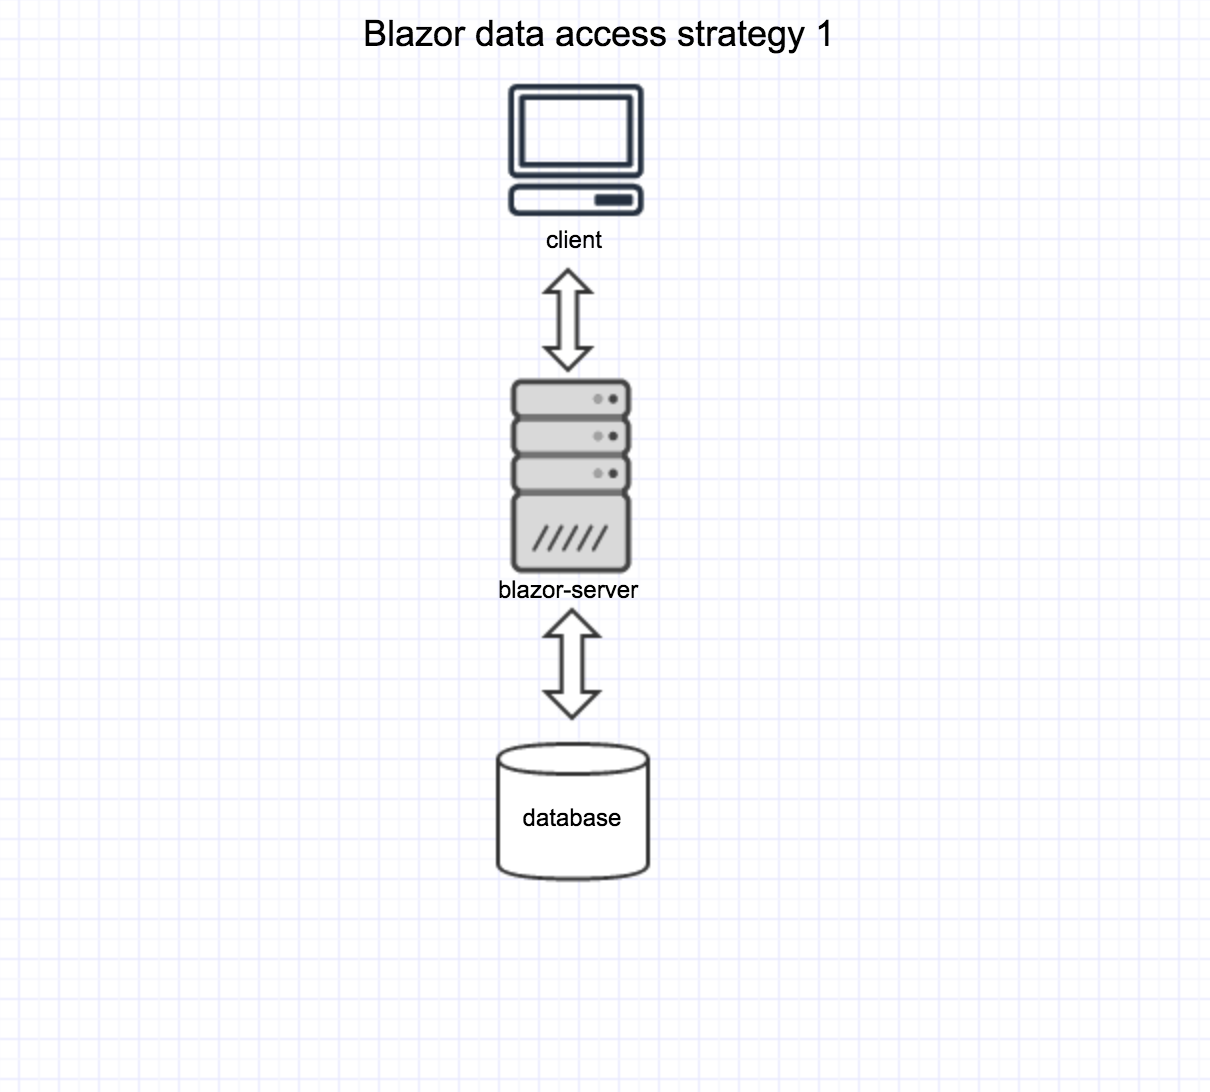
\includegraphics[width=150mm]{data/ds1.JPG}
\caption{Blazor data access strategy 1 }
\label{blabla}
\end{figure}


Here, the client calls the server application(Blazor application). Here, we utilize SignalIR, which is used to connect the client and server and exchange data between them.
Figure 7 shows the example of the architecture, where the server has access to the database and can directly communicate with it.
 We can use this type of architecture when we do not plan to make any future changes in our application.\\
However, we know that it is possible to change our application from Blazor Server to Blazor WebAssembly, it is better to use another architecture, because with this one we would have to do a lot more work.
The is the option when the Blazor application will always be running on the server.\\
Another option  is to use the RESTful service in our application.
In this case, the communication between the server and database is different.
The Blazor application calls the RESTful service. Afterwards, this service calls the database via the Entity Framework Core.\\
\begin{figure}[H]
\centering
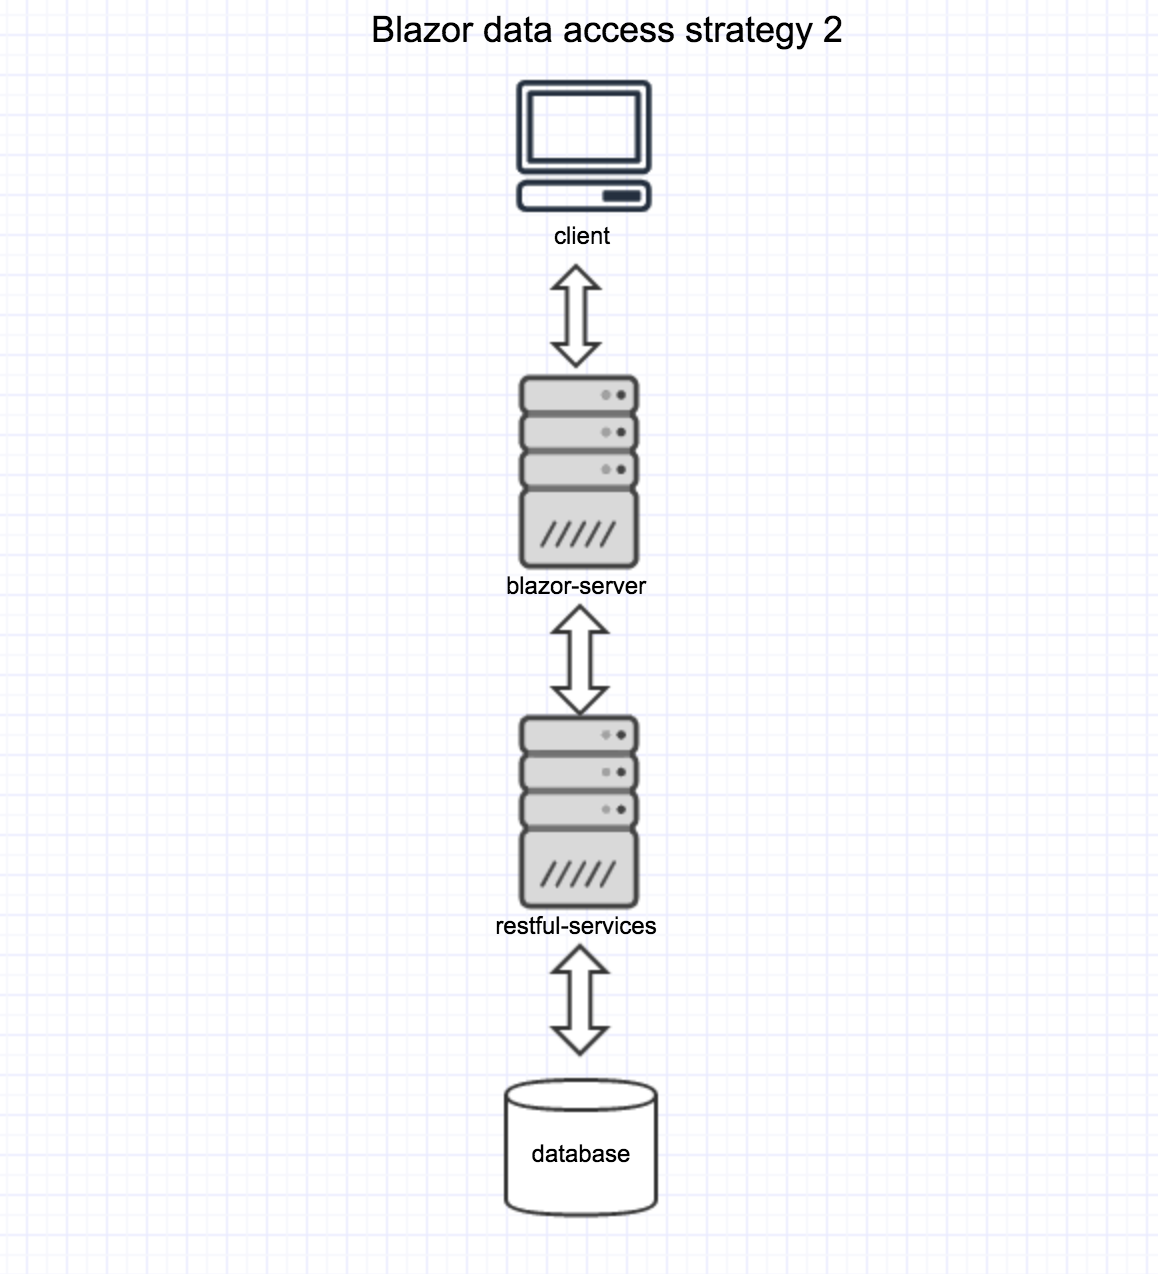
\includegraphics[width=150mm]{data/ds2.JPG}
\caption{Blazor data access strategy 2}
\label{blabla}
\end{figure}
The benefit of this model (depicted in Figure 8) is that we can use this code for both Blazor models: Blazor Server and Blazor WebAssembly with only small changes. This model is more flexible.


Comparing these two options and knowing that in the future it is possible to make a transition to the client side version, we will use the RESTful service model
RESTful APIs use the Representational State Transfer pattern to create an API(Application Programming Interface). 

\subsection{Setup for Blazor}
To use the Blazor framework it is necessary to install :\\
\begin{itemize}
\item \textbf{.NET Core SDK 3.1 or later} from \url {http://dotnet.microsoft.com/download}
\item \textbf{Visual Studio 2019} from \url {https://visualstudio.microsoft.com/downloads/}
\end{itemize}

\section{Proof of Concepts }
%/**
%determine whether an idea can be turned into a reality\\
%test if the idea is viable and explore 
%\\
%how the proposed product or service will support organizational goals\\
%*/

In this section, we want to collect information about the technologies which we chose. We also want to describe our first experience with these technologies.

As mentioned in the previous section for our project, we chose the Blazor framework.

Does it suit us? Does it meet the requirements of the system?
How popular is it? Is its popularity growing or falling? Popularity is an important indicator of the effectiveness of this framework.\\
\subsection{Popularity of Blazor}
Based on information from the Internet, web frameworks like  React, Angular, Vue.js are the most popular today. \\


In Figure 9 we have used the GitHub framework comparison to compare the history of stars of the most popular frameworks and Blazor. \cite{starhistory}

 \begin{figure}[H]
\centering
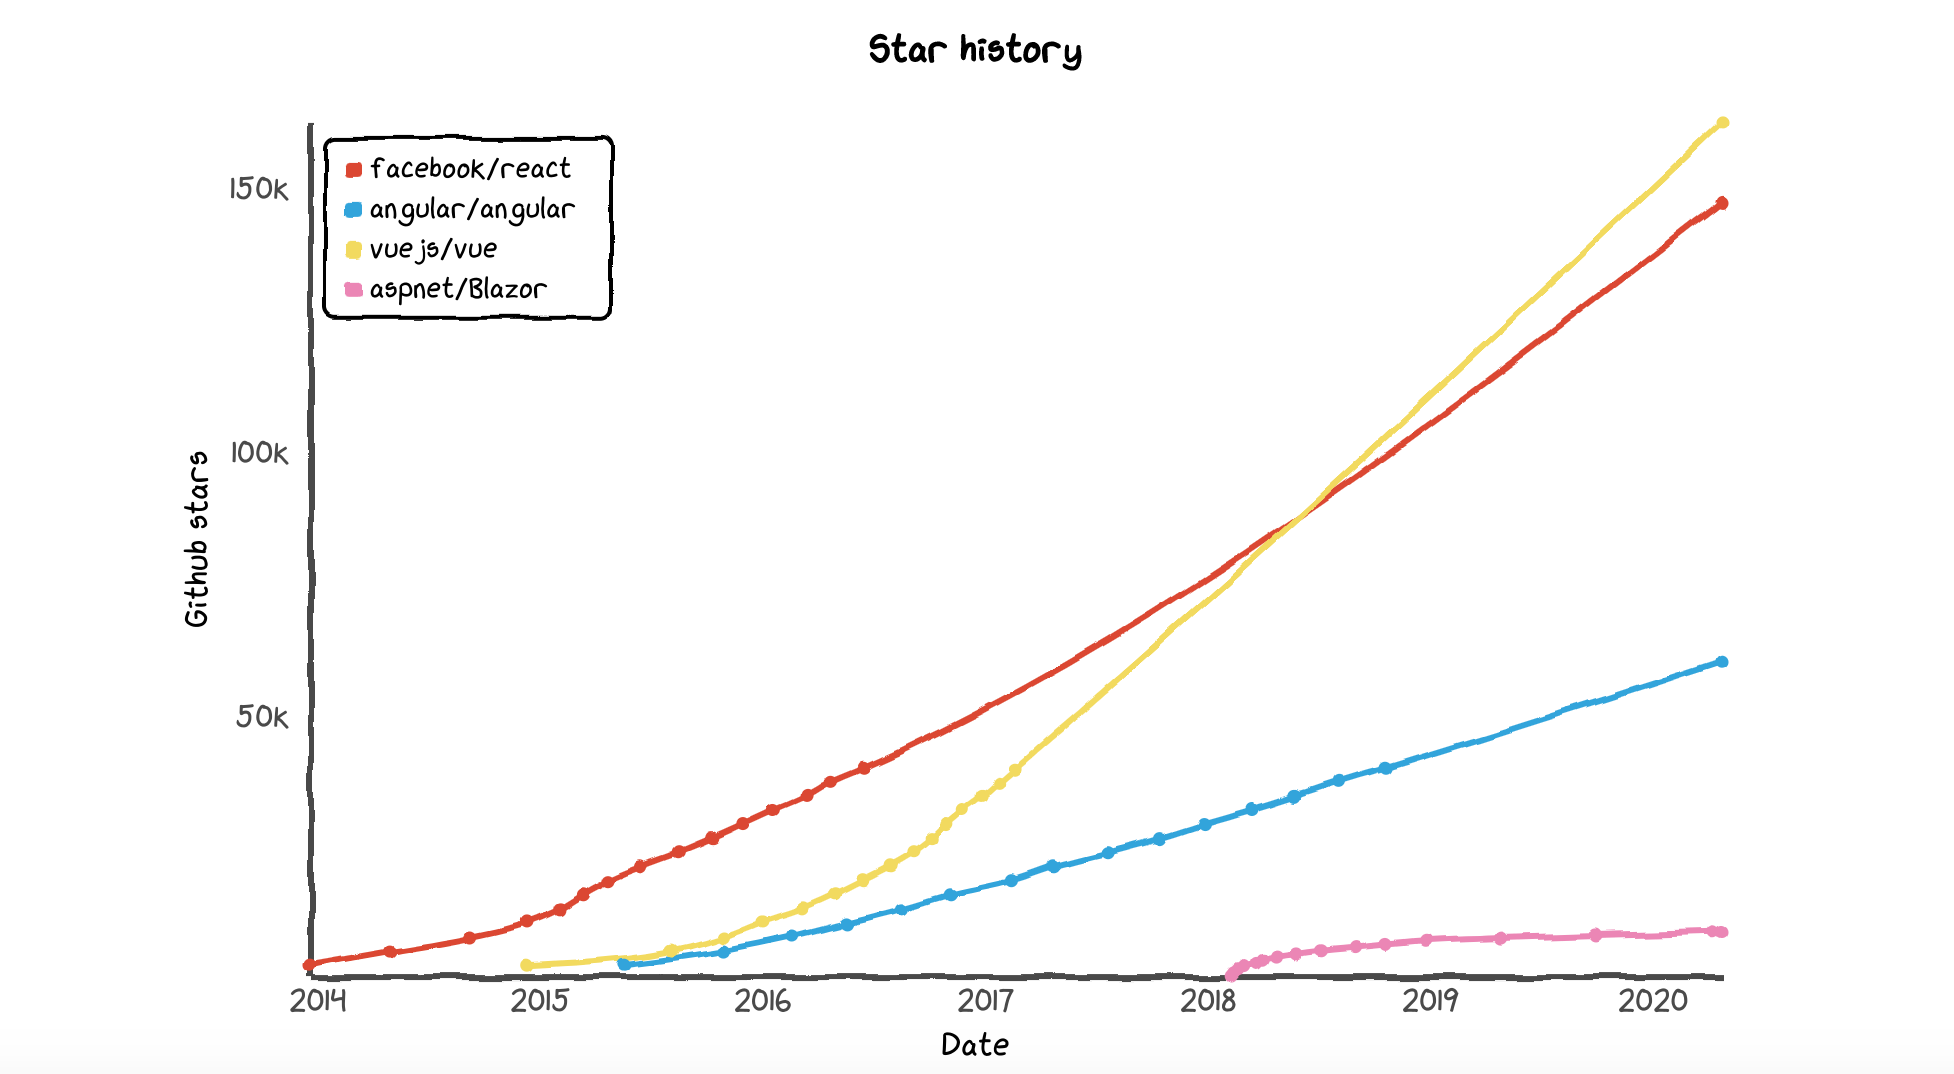
\includegraphics[width=150mm]{graph/star-history-all.JPG}
\caption{History of stars comparison of frameworks}
\label{blabla}
\end{figure}

If we compare the Blazor framework to these three most popular frameworks, we can see that it has a smaller number of stars, but this is due primarily to the fact that Blazor is a young framework.\\
If we consider Blazor separately, we see a progressive increase in popularity.

 \begin{figure}[H]
\centering
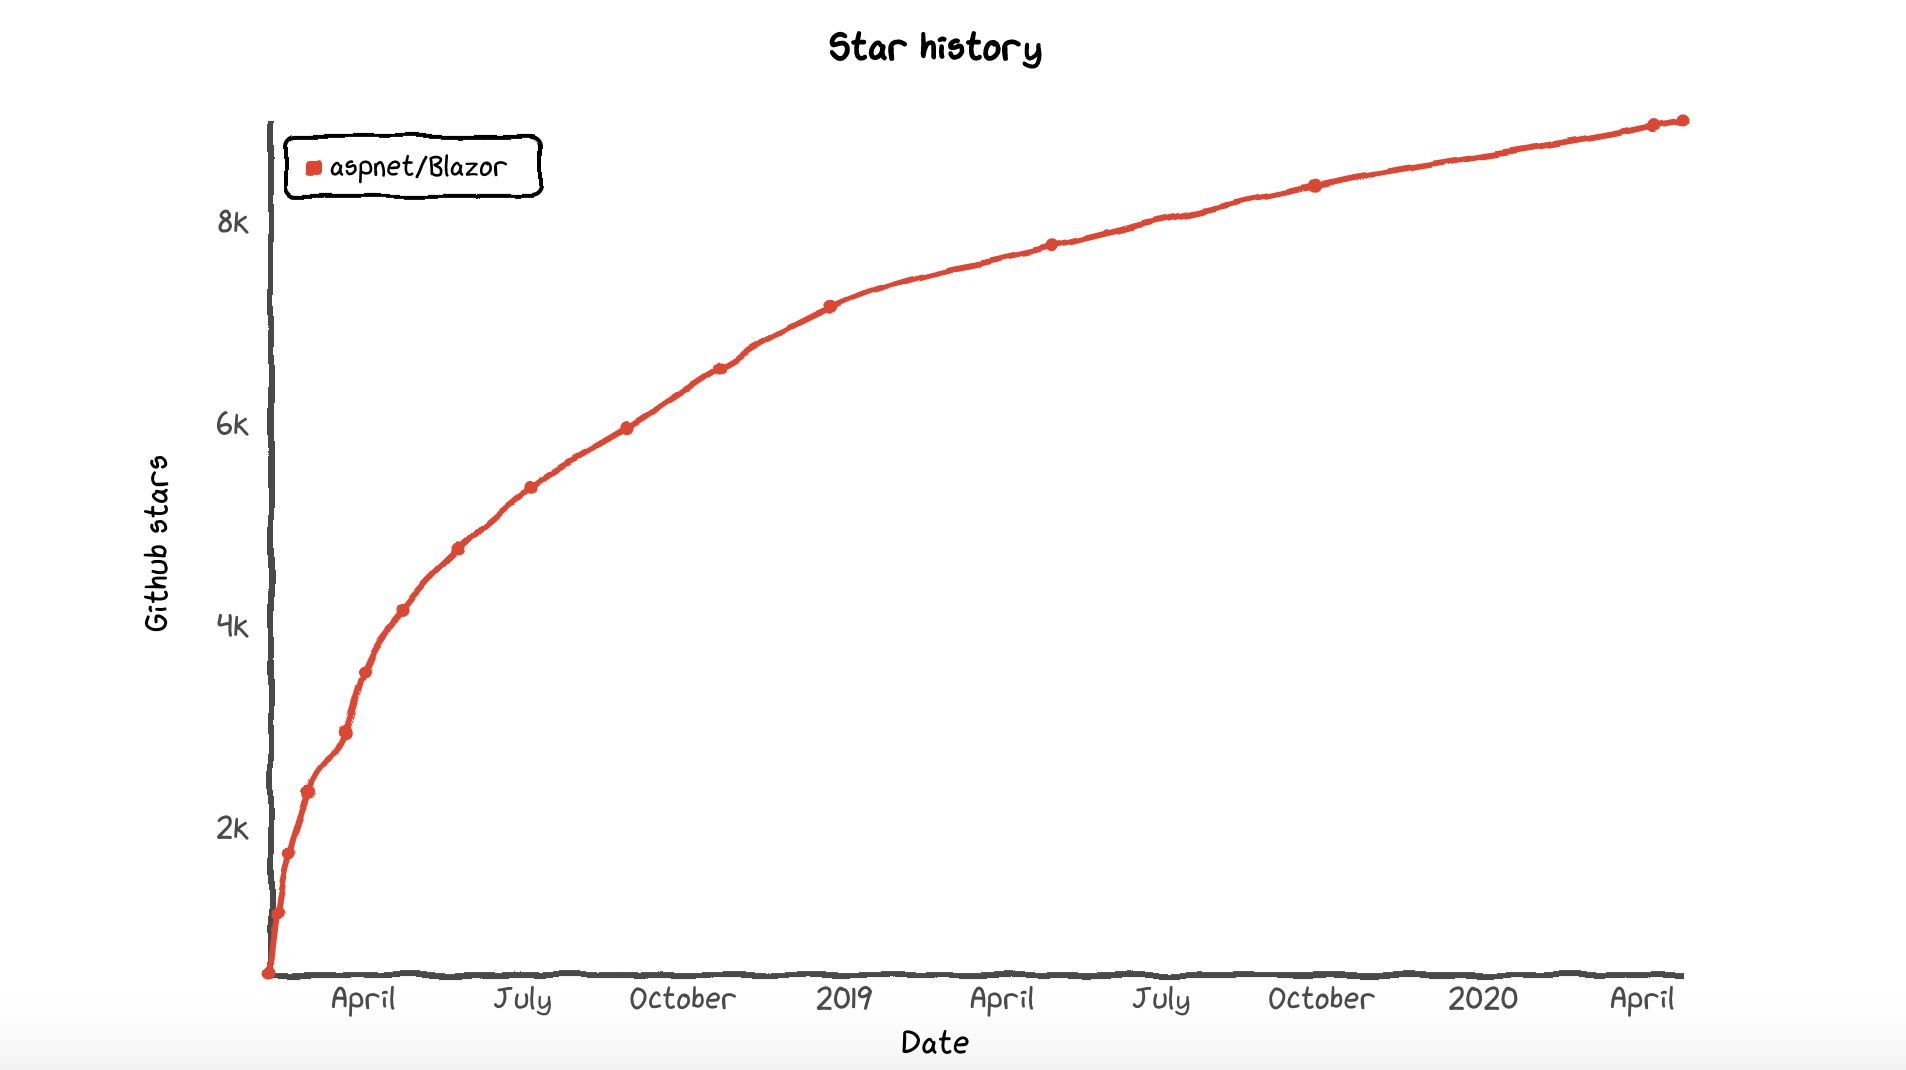
\includegraphics[width=150mm]{graph/star-history-blazor.JPG}
\caption{History of stars of Blazor framework}
\label{blabla}
\end{figure}

%%%%%%%%% interest

Another tool that we using to see the popularity of the Blazor is Google Trends. The Figure 11 shows us which frameworks are the most searched for in Google Search. \cite{interest-over-time}
 \begin{figure}[H]
\centering
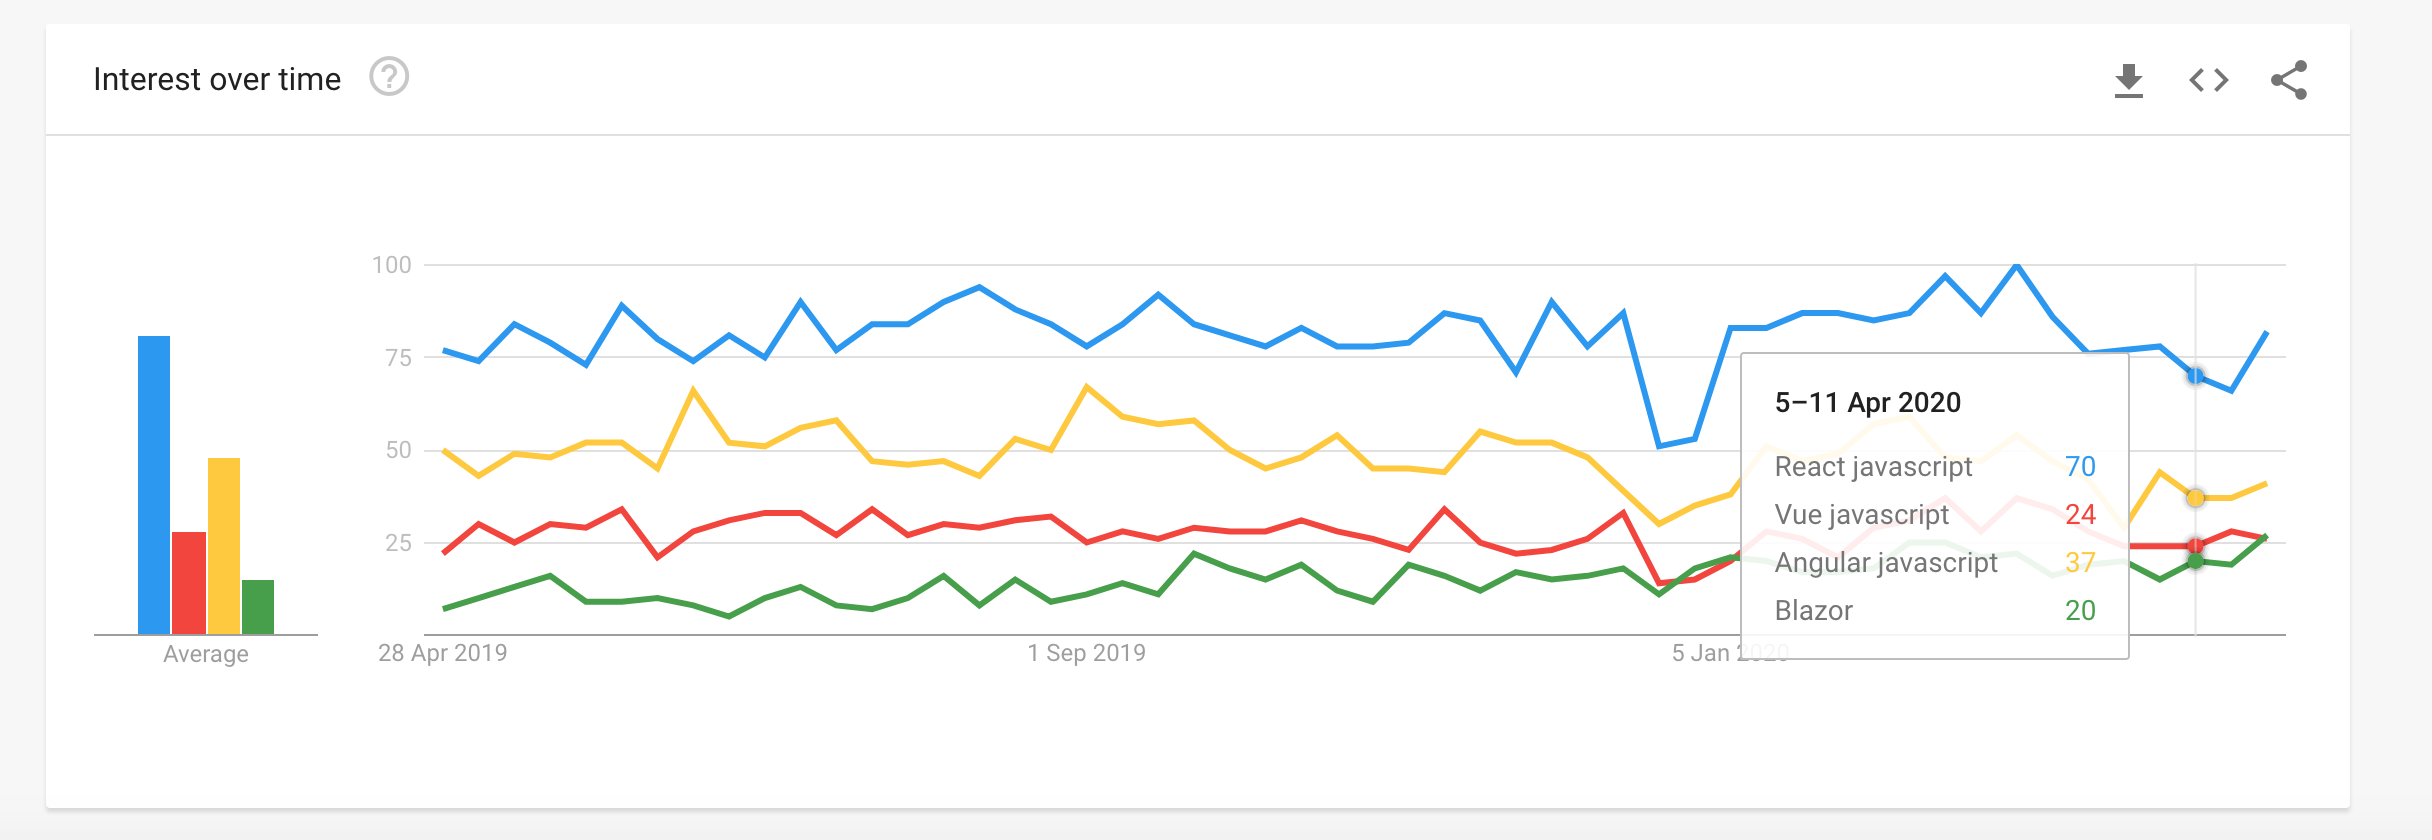
\includegraphics[width=150mm]{graph/interest-all.JPG}
\caption{Interest over time of frameworks}
\label{blabla}
\end{figure}

As we can see, the React.js is the most popular framework in Google Search. Then comes Angular, followed by VueJs.
 Blazor is the youngest framework, but people are often interested in it.
The Figure 12 shows us how the popularity of Blazor significantly increased in recent years. Which is an important positive indicator.


 \begin{figure}[H]
\centering
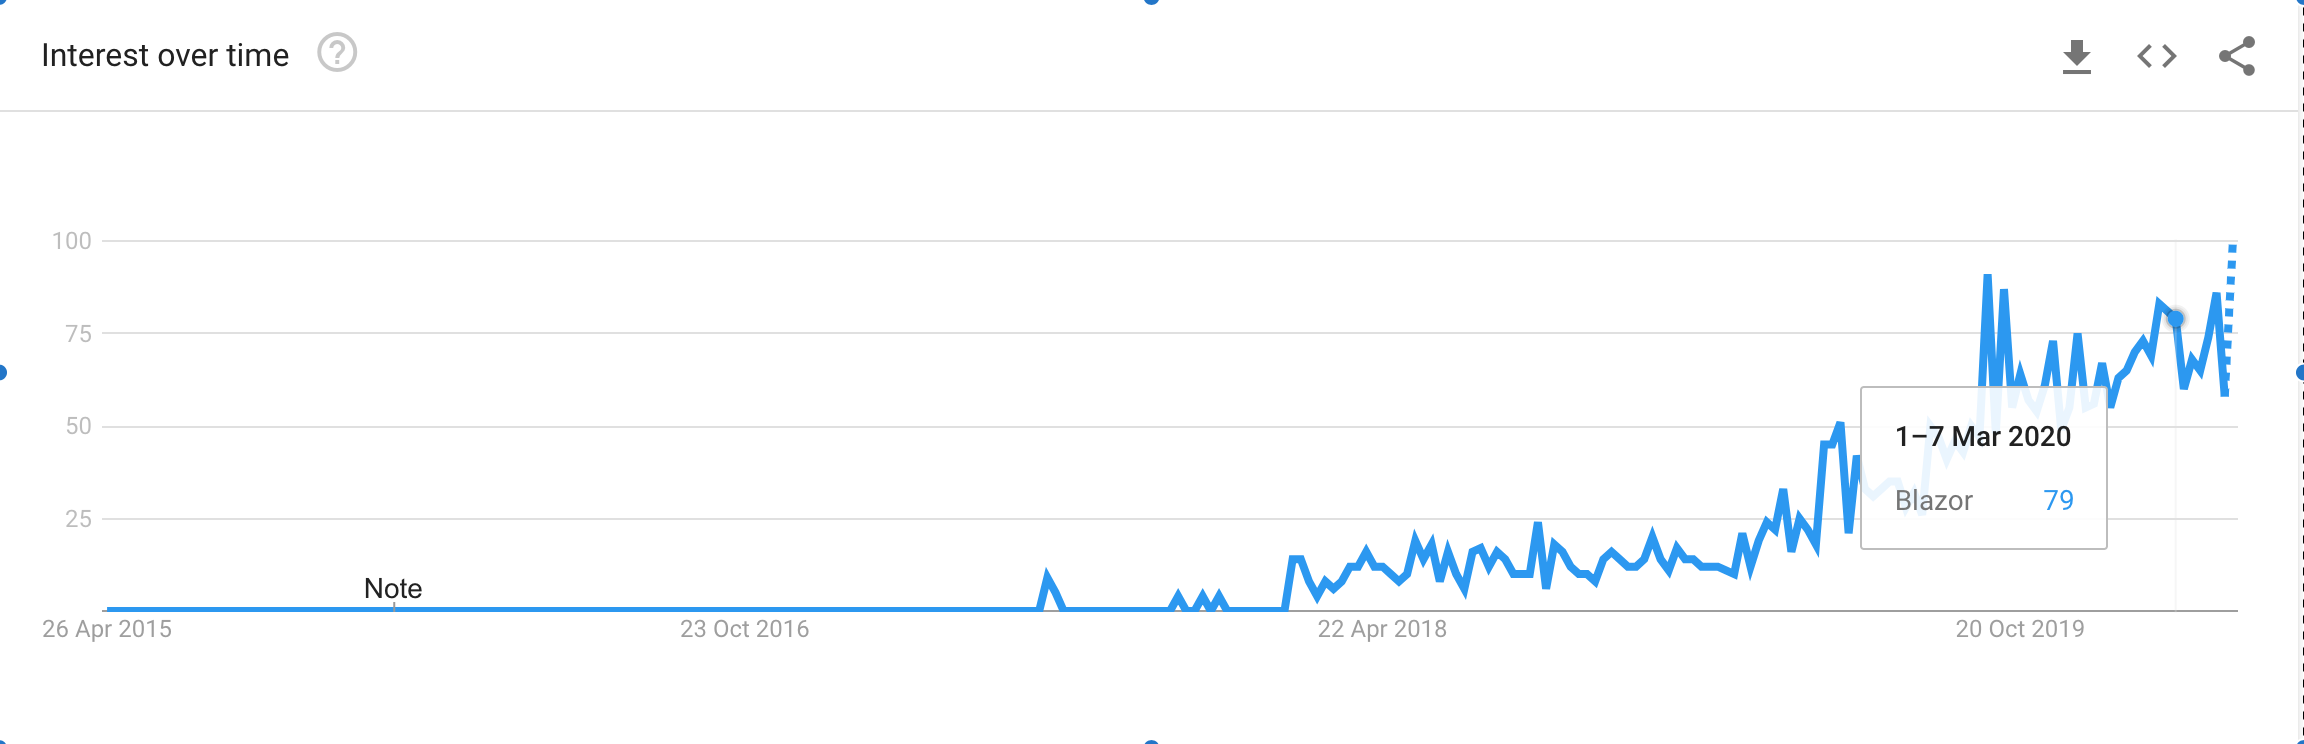
\includegraphics[width=150mm]{graph/interest-blazor.JPG}
\caption{Interest over time in Blazor framework}
\label{blabla}
\end{figure}


\subsection{Testing the Proposed Project Structure with Selected Technologies}
Before starting with the main project, we have tested Blazor on small projects. We tried the WebAssembly client side model and the server side model. 
Then we have started with the main project and defined the use cases that we will implement as part of this project. All documentation for the implementation is in a separate document \textbf{" Visual Review In Initial Phase of Project.docx".}\\
Our experience with these technologies is quite positive. We managed to do the tasks in the allotted time frame. We have learned a lot and there is still a lot to learn, but despite all this, the result is nevertheless satisfactory.

\newpage
\subsection{Summary of Proof of Concepts }


There are so many different possibilities to implement web applications using frameworks.
When choosing a framework for our project, we based our decision on factors that are more suitable for us, i.e. functions that we need, architecture, programming language.
We decided to create a project using the Blazor framework. It allows us to create a server-side and client-side applications using  C\#. 
We did research on the popularity of Blazor. Finally, to create a project using the Blazor framework. Summing up all this, we want to say that Blazor's popularity is growing, working with the Blazor framework is interesting and easy,  the Blazor UI is pleasant to look at. We do not need to create separate model classes for the back-end and front-end. The same model classes are shared with both client and server. 
%And most importantly, these are our conclusions from our experience with this framework.
\\


\section{Work Plan}
  		\subsection{Effort Estimation}
  		
  		Project 2  is designed as a 4 ECTS module. This corresponds to a workload of 120 hours. When we are working on a project, we always record our hours of work in an Excel table.
 At the end of the project, we will compare this time with the time allotted for the project. 		
  		
  		
  		
  		
  		
 	    \subsection{Scrum}  	
 	    The foundation of the project organization was Scrum.
 	    Some principles of Scrum could not be achieved since they need a group of more than two people. 
 	    Our work was based on the principles of Scrum like the Empirical Process of Control, the core of Scrum, self-organization, value-based prioritization, etc.
 	    The Empirical Process of Control includes three main ideas, namely transparency, inspection, and adaptation. \\
 	    Transparency: The work is carried out in full trust of all parties involved. Everyone has the courage to keep each other up to date with both good and bad news. \\ 
 	    Inspection: Inspection is carried out by every one in the Scrum Team. The team openly shows the product at the end of each Sprint.			 \\
 	    Adaptation: The team asks constant questions about the progress of work, whether we are on the right way. Depending on this, we can adapt an existing product.		 \\
 	    
 	    At the beginning of the project, we have discussed and estimated all the work that needs to be done. 
 	    Meetings between supervisor and developer are weekly and sometimes bi-weekly.
 	    Each meeting includes a discussion about what has been achieved 
 	    since the tasks have been assigned, what can be improved, and scheduling of future tasks.
 	    
 	    
 	    
 	    
 	    
  		\subsubsection{Scrum Roles}
  		\begin{itemize}
  		\item Product Owner: Mr. Pfahrer
  		\item Development Team: Shiryagina Kristina
  		\item Scrum Master: Shiryagina Kristina
  		
  		\end{itemize}
  	    \subsubsection{Scrum Plan}
  	    To discuss the project, were weekly and biweekly meetings held . They included personal meetings, and then meetings using Microsoft Teams. The meetings consisted of:
  	    \begin{itemize}
  	    \item Sprint Review. It includes a show of work and its discussion.
  	    \item Sprint Planning. It includes the scheduling of future tasks.
  	    \item Sprint Retrospective. It includes discussion about what went well and what went wrong, what we should do differently. 
  	    \end{itemize}
  		\subsubsection{Scrum Artefacts }
  		
  		\subsubsection{Sprints}
  		
	The sprints covered a one week period. At the end of each sprint, there was a discussion with the supervisor.

In Table 11 is an overview of what was achieved in which sprint.

\begin{table}[H]
\begin{center}
\begin{tabular}{| p{2.5cm}| p{12cm} |}
\hline
\rowcolor{LightCyan}
\textbf{Sprint} & \textbf{Goals and Achievements} \\
\hline

1                   &             
\begin{itemize}
\item Make a proposal
 \item Customer Problem Statement description
 \item Asp.net core tutorials
 \item Requirement engineering, User Stories


 \end{itemize}\\ \hline
 
2                &             
\begin{itemize}
 \item Requirement engineering, Functional Requirements 
 \item Asp.net core tutorials
 \item Problem Statement: Excel vs Web application


 \end{itemize}\\ \hline
 3                 &             
\begin{itemize}
\item Requirement engineering, Non-Functional Requirements
 \item Actors and goals
 \item Define the use cases
 \item Small employee-management asp.net core project


 \end{itemize}\\ \hline
 4                   &             
\begin{itemize}
 \item Small employee-management asp.net core project
 \item Use case diagram
 \item Blazor tutorials
\end{itemize}\\ \hline
 
  5              &             
\begin{itemize}
 \item Domain model
 \item Blazor tutorials
 \item Blazor WebAssembly CRUDApp small project


 \end{itemize}\\ \hline
 

 
 

 \end{tabular}
\end{center}
\caption{Sprints}
\label{table2}
\end{table}

\pagebreak

\begin{table}[H]
\begin{center}
\begin{tabular}{| p{2.5cm}| p{12cm} |}
\hline
\rowcolor{LightCyan}
\textbf{Sprint} & \textbf{Goals and Achievements} \\
\hline

6                &             
\begin{itemize}
 \item Update domain model
 \item Add attributes to the domain model
 \item Add new use cases


 \end{itemize}\\ \hline
 
  7                 &             
\begin{itemize}
 \item  Learn about Server side model of Blazor
 \item Small  project to-do list with Blazor
 \end{itemize}\\ \hline
 
  8                 &             
\begin{itemize}
 \item Make BPMN2 process diagram with entities.
 \item Update Excel vs Web Application diagram, add table
 \end{itemize}\\ \hline
 
  9                 &             
\begin{itemize}
 \item User interface
 \item  Create services, components of Blazor
 
\end{itemize}\\ \hline
 
  10                &             
\begin{itemize}
 \item Update BPMN
 \item Start Chapter Proof of Concepts
 
 \item Start project, Add initial structure of project, Add model classes


 \end{itemize}\\ \hline
 
  11                &             
\begin{itemize}
 \item Project: add database, add API project, add repositories and controller class
 \item System Architecture and Design
 \item Make table of comparison of Blazor with the most popular framework


 \end{itemize}\\ \hline
 
 
 \end{tabular}
\end{center}
\caption{Sprints}
\label{table2}
\end{table}
 
 
 \pagebreak

\begin{table}[H]
\begin{center}
\begin{tabular}{| p{2.5cm}| p{12cm} |}
\hline
\rowcolor{LightCyan}
\textbf{Sprint} & \textbf{Goals and Achievements} \\
\hline
 
 
  12               &             
\begin{itemize}
\item Technologies
 \item Choose the use case for the programming part of the project
 

 \end{itemize}\\ \hline
 
  13                &             
\begin{itemize}
\item Project, Add pages to the Blazor project
\item Make a description of my experience,which I have acquired while doing this project. 


 \end{itemize}\\ \hline
  14                &             
\begin{itemize}
 \item Make a document - code review of initial steps of project
 \item Describe components, services, controller and other important components of project in document
\end{itemize}\\ \hline
 
 15                 &             
\begin{itemize}
 \item Project: edit Lecturer and view Lecturer use cases
 \item Describe work management


 \end{itemize}\\ \hline
 16               &             
\begin{itemize}
 
 \item  Implement delete and search functions on front-end
 \item  Add conclusion  part of the report. 


 \end{itemize}\\ \hline
 17               &             
\begin{itemize}
 \item Prepare report and review documents for the final delivery
 \item Prepare all documents and project for the final delivery
 \item Add necessary data for the glossary, acronyms ,references.


 \end{itemize}\\ \hline
 
\end{tabular}
\end{center}
\caption{Sprints}
\label{table2}
\end{table}



\section{Conclusions and Future Work}
%   \subsubsection{Summary}
\subsection{Conclusions}
   The purpose of this project is to prepare the necessary environment for the  undergraduate project "Planning of the assignments information system(PLANA)" web application.\\
   To achieve this goal the following tasks were completed.
   \begin{itemize}
    
   \item \textbf{ Requirements engineering } \\
   We determined the use cases of the system, actors, and all the necessary conditions that the system should satisfy.
   \item \textbf{ Domain Analysis }\\
  We distinguished concept classes, designated interactions between them and created a domain model with its attributes.
   \item \textbf{ Architecture and Design of System}\\
   We have chosen the  \textbf{client-server} model for our system. We determined the subsystems and selected the MS SQL database.
   \item \textbf{ Exploration of Technologies } \\
   We did a research on ASP.NET Core Blazor and we also 
     made small projects based on this technology . They were executed 	 successfully.
    The initial structure of the project has been created and the CRUD functions  for lecturers have been implemented.
    \end{itemize}
    
    
    The conclusions that we want to draw are that the technologies that we tried for the project are fully suited to our goals. 
    	The project will continue to utilize technologies such as ASP.NET Core Blazor.
    	The project structure has been defined, i.e the environment is prepared for the subsequent implementation of the project.
    	\subsection{Future Work		}
    	As we mentioned above the bachelor thesis is a continuation and expansion of this project, for which  we are planning the following future extensions:
    \begin{itemize}
    \item [$-$]The embodiment of our intended use cases
    		\begin{itemize}
   		 \item  Implementation of relationships between model classes
  		  \item Creating the necessary controllers and repositories
   			 \item Creating an easy to understand and user friendly interface
  		  \
    \end{itemize}
	
	\item [$-$]  System Testing implementation 
			\begin{itemize}
			\item Unit-Tests
			\item Check-list for front-end
			\item Postman for CRUD operation of controllers
			\item Database test
			\item Compatibility test
			\item Usability test
			
		\end{itemize}
  
\end{itemize}	
    	The final product should be a easy to use, easy to understand and user friendly application that will fulfil the main goal - "Planning of assignments for lecturers", which will be implemented on the latest technology - ASP.NET Core Blazor.
%  \subsubsection{Interpretation }
%  
%  \subsubsection{Outlook}



\newpage

%% print the bibliography and add the section to the table of content

\printbibliography[heading=bibintoc]

Document structure  \\
\url{https://www.ece.rutgers.edu}

\pagebreak









  	
  
  	

  	
  	
  	
  
  	
  	
  	
  
  	
  	
  
  	


  	





	
	
	




 









 

 




%%%%%%%%%% aditional report elements %%%%%%%
%\subsection{Interface viewpoint}
%\textbf{\textit{DESIGN CONCERNS}}
%\\
%The interface viewpoint provides information about how I want to design  user interface. \\
%
%%todo: make and put here the welcome page 
%After downloading the application, and running the first time, the user will be directed to Welcome page.\\
%
%\textbf{\textit{Design elements.}}
%
%
%
%
%
%
%
%\subsection{Feasibility}
%\subsubsection{Technical Feasibility}
%This project is a web-based application. The main technologies and tools:
%\begin{itemize}
%  	\item
%  	\item
%  	\item GIT  2.20.1.windows.1
%  	\item GIFFY(DIAGRAM DRAWING TOOL)
%  	\item LATEX 3.14159265-2.6-0.99999 (TeX Live 2019/dev/Debian)
%
%  
%  	
%  	\end{itemize}
% \subsubsection{Financial Feasibility}
% Being a web application  will have a hosting cost.
% \subsubsection{Resource and Time Feasibility}
% \begin{itemize}
% \item Laptop (programming device)
% \item Hosting
% \item Programming tools
% \end{itemize}


















                      
        
    


   

   
    
   
  

\section{Protocol}
\textbf{\textit{Frequency: (weekly) \\
Meeting length: (60 minutes)}}\\

Agenda

\begin{itemize}
  	\item Demo and Discuss Deliverable(Demo)
  	\item Planning next Goals(Plan)
  	\item Lessons learned (Lessons)
  	\item Date, time of the next meeting(next meeting)
 \end{itemize} 	


\textbf{\textit{Report from  26.02.20 }}\\
Plan\\
Future goals are: 
\begin{itemize}


	\item Requirements 
	\item asp.net core tutorials 
\end{itemize}	
Lessons learned\\

Next Meeting: .....\\
%%%%%%%%%%%%%%%%%%%%%%%%%%%

\textbf{\textit{Report from 23.03.20  }}\\
Plan\\
Future goals are: 
\begin{itemize}

  \item Domain model update
	\item Add attributes to the domain model
	\item Describe actors 
	\item Add 2 more use cases 
	\item Change use case diagram, add requirements for these new use cases
	\item Add changes to problem statement and make it more understandable.
\end{itemize}	
Lessons learned\\

Next Meeting: 30.03.20\\
%%%%%%%%%%%%%%%%%%%%%%%%%%%%

%%%%%%%%%%%%%%%%%%%%%%%%%%%

\textbf{\textit{Report from 30.03.20  }}\\
Plan\\
Future goals are: 
\begin{itemize}

\item Make BMN2 process diagram with entities. This diagram is a good tool to show who does what.
	\item  In the Problem statement, transform the information (Excel in comparison to the web app) from a diagram to a table.
	\item FURPS+ (source information)
	\item Better describe the problem statement
	\item Change uc6 (delete Institute-manager actor or extend uc6 with uc6.1 "list of research assignments")
\item Domain model will be discussed with the supervisor 	
	
\end{itemize}	
Lessons learned\\ Important to give information in an easy to understand/read format, so that the reader can understand it without reading the report several times, e.g. table form.

Next Meeting: 14.04.20(09:00-10:00)\\
%%%%%%%%%%%%%%%%%%%%%%%%%%%%

%%%%%%%%%%%%%%%%%%%%%%%%%%%

\textbf{\textit{Report from 14.03.20  }}\\
Plan\\
Future goals are: 

\begin{itemize}


	\item Change bpmn, first create a process of s. director, then the joint process of plan managing
	\item Add Chapter Proof of Concepts (prototyping)
	\item Start document chapters: 6-8
	\item Start programming
\end{itemize}	
Lessons learned\\

Next Meeting: 20.04.20(09:00-10:00)\\
%%%%%%%%%%%%%%%%%%%%%%%%%%%%

%%%%%%%%%%%%%%%%%%%%%%%%%%%

\textbf{\textit{Report from   20.04.20}}\\
Plan\\
Future goals are: 
\begin{itemize}
	\item	Continue to describe chapters 6-8(change 7<->8) For chapter 7 (poc) make a 
	table with comparing different popular frameworks with blazor
	\item Implement model classes for PLANA
\end{itemize}	
Lessons learned\\

	

Next Meeting: 27.04.20(09:00-10:00)\\
%%%%%%%%%%%%%%%%%%%%%%%%%%%%

\textbf{\textit{Report from  27.04.20 }}\\
Plan\\
Future goals are: 
\begin{itemize}


	\item For a document: 
	\begin{enumerate}
	\item Determine what exactly will we program in project 2
	\item Describe it in the separeted document "Visual Review In Initial Phase of Project"
	\item After trying to write code and implement several functions, describe it and write in the conclusions our experience. Will it be easy to create the application, or are there some problems which we will have to address before proceeding with the bachelor thesis.
	\end{enumerate}
	\item
\end{itemize}	
Lessons learned: How to make Proof of concepts\\

Next Meeting: 11.05.20\\
%%%%%%%%%%%%%%%%%%%%%%%%%%%%

\textbf{\textit{Report from  11.05.20 }}\\
Plan\\
Future goals are: 
\begin{itemize}


	\item Put more information regarding implementation description of overview document, add diagram project dependencies. Describe component, services, controller, how they interact with each other.
	\item Add the work plan in the main document.
	\item Continue to  code the project 
\end{itemize}	
Lessons learned\\ Try to see the content of the documentation from the side of the person who is reading the report. Putting the diagrams in the document makes it easier to understand the given information.

Next Meeting: 25.05.20\\

%%%%%%%%%%%%%%%%%%%%%%%%%%%%
\textbf{\textit{Report from 25.05.20  }}\\
Plan\\
Future goals are: 
\begin{itemize}


	\item Implement delete and search function on front-end
	\item Write the conclusion of the report . Prepare report and review documents for the final delivery.
	\item Prepare all documents and project for the final delivery
\end{itemize}	
Lessons learned\\
soft-delete\\
Next Meeting: 08.06.20\\

%%%%%%%%%%%%%%%%%%%%%%%%%%%%
\textbf{\textit{Report from  08.06.20 }}\\
Plan\\
Future goals are: 
\begin{itemize}


	\item Finish writing code
	\item Prepare all documents and project for the final delivery
\end{itemize}	
Lessons learned\\

%Next Meeting: .....\\

%%%%%%%%%%%%%%%%%%%%%%%%%%%%





\end{document}





